
\documentclass{article}
%%%%%%%%%%%%%%%%%%%%%%%%%%%%%%%%%%%%%%%%%%%%%%%%%%%%%%%%%%%%%%%%%%%%%%%%%%%%%%%%%%%%%%%%%%%%%%%%%%%%%%%%%%%%%%%%%%%%%%%%%%%%%%%%%%%%%%%%%%%%%%%%%%%%%%%%%%%%%%%%%%%%%%%%%%%%%%%%%%%%%%%%%%%%%%%%%%%%%%%%%%%%%%%%%%%%%%%%%%%%%%%%%%%%%%%%%%%%%%%%%%%%%%%%%%%%
\usepackage{eurosym}
\usepackage{amsmath}
\usepackage{amssymb}
\usepackage{amsfonts}
\usepackage{graphicx}
\usepackage[utf8]{inputenc}
\usepackage[english]{babel}
\usepackage{chngcntr}
\usepackage{apptools}

\setcounter{MaxMatrixCols}{10}
%TCIDATA{OutputFilter=LATEX.DLL}
%TCIDATA{Version=5.50.0.2960}
%TCIDATA{<META NAME="SaveForMode" CONTENT="1">}
%TCIDATA{BibliographyScheme=Manual}
%TCIDATA{Created=Saturday, August 10, 2013 22:44:33}
%TCIDATA{LastRevised=Wednesday, June 15, 2016 23:20:42}
%TCIDATA{<META NAME="GraphicsSave" CONTENT="32">}
%TCIDATA{<META NAME="DocumentShell" CONTENT="Standard LaTeX\Blank - Standard LaTeX Article">}
%TCIDATA{CSTFile=40 LaTeX article.cst}

%\newtheorem{theorem}{Theorem}
%\newtheorem{acknowledgement}[theorem]{Acknowledgement}
%\newtheorem{algorithm}[theorem]{Algorithm}
%\newtheorem{assumption}[theorem]{Assumption}
%\newtheorem{axiom}[theorem]{Axiom}
%\newtheorem{case}[theorem]{Case}
%\newtheorem{claim}[theorem]{Claim}
%\newtheorem{conclusion}[theorem]{Conclusion}
%\newtheorem{condition}[theorem]{Condition}
%\newtheorem{conjecture}[theorem]{Conjecture}
%\newtheorem{corollary}[theorem]{Corollary}
%\newtheorem{criterion}[theorem]{Criterion}
%\newtheorem{definition}[theorem]{Definition}
%\newtheorem{example}[theorem]{Example}
%\newtheorem{exercise}[theorem]{Exercise}
%\newtheorem{lemma}[theorem]{Lemma}
%\newtheorem{notation}[theorem]{Notation}
%\newtheorem{problem}[theorem]{Problem}
%\newtheorem{proposition}[theorem]{Proposition}
%\newtheorem{remark}[theorem]{Remark}
%\newtheorem{solution}[theorem]{Solution}
%\newtheorem{summary}[theorem]{Summary}


\newtheorem{theorem}{Theorem}[section]
\newtheorem{corollary}{Corollary}[theorem]
\newtheorem{lemma}[theorem]{Lemma}
\newtheorem{definition}[theorem]{Definition}
\newtheorem{remark}[theorem]{Remark}
\newtheorem{assumption}[theorem]{Assumption}
\newtheorem{notation}[theorem]{Notation}
\newtheorem{fact}[theorem]{Fact}
\newtheorem{proposition}[theorem]{Proposition}

\newenvironment{proof}[1][Proof]{\noindent\textbf{#1.} }{\ \rule{0.5em}{0.5em}}
\setlength{\topmargin}{0cm}
\setlength{\textheight}{21.5cm}
\setlength{\textwidth}{16.5cm}
\setlength{\oddsidemargin}{0cm}
\renewcommand{\baselinestretch}{1}
% Macros for Scientific Word 2.5 documents saved with the LaTeX filter.
%Copyright (C) 1994-95 TCI Software Research, Inc.
\typeout{TCILATEX Macros for Scientific Word 2.5 <22 Dec 95>.}
\typeout{NOTICE:  This macro file is NOT proprietary and may be 
freely copied and distributed.}
%
\makeatletter
%
%%%%%%%%%%%%%%%%%%%%%%
% macros for time
\newcount\@hour\newcount\@minute\chardef\@x10\chardef\@xv60
\def\tcitime{
\def\@time{%
  \@minute\time\@hour\@minute\divide\@hour\@xv
  \ifnum\@hour<\@x 0\fi\the\@hour:%
  \multiply\@hour\@xv\advance\@minute-\@hour
  \ifnum\@minute<\@x 0\fi\the\@minute
  }}%

%%%%%%%%%%%%%%%%%%%%%%
% macro for hyperref
\@ifundefined{hyperref}{\def\hyperref#1#2#3#4{#2\ref{#4}#3}}{}

% macro for external program call
\@ifundefined{qExtProgCall}{\def\qExtProgCall#1#2#3#4#5#6{\relax}}{}
%%%%%%%%%%%%%%%%%%%%%%
%
% macros for graphics
%
\def\FILENAME#1{#1}%
%
\def\QCTOpt[#1]#2{%
  \def\QCTOptB{#1}
  \def\QCTOptA{#2}
}
\def\QCTNOpt#1{%
  \def\QCTOptA{#1}
  \let\QCTOptB\empty
}
\def\Qct{%
  \@ifnextchar[{%
    \QCTOpt}{\QCTNOpt}
}
\def\QCBOpt[#1]#2{%
  \def\QCBOptB{#1}
  \def\QCBOptA{#2}
}
\def\QCBNOpt#1{%
  \def\QCBOptA{#1}
  \let\QCBOptB\empty
}
\def\Qcb{%
  \@ifnextchar[{%
    \QCBOpt}{\QCBNOpt}
}
\def\PrepCapArgs{%
  \ifx\QCBOptA\empty
    \ifx\QCTOptA\empty
      {}%
    \else
      \ifx\QCTOptB\empty
        {\QCTOptA}%
      \else
        [\QCTOptB]{\QCTOptA}%
      \fi
    \fi
  \else
    \ifx\QCBOptA\empty
      {}%
    \else
      \ifx\QCBOptB\empty
        {\QCBOptA}%
      \else
        [\QCBOptB]{\QCBOptA}%
      \fi
    \fi
  \fi
}
\newcount\GRAPHICSTYPE
%\GRAPHICSTYPE 0 is for TurboTeX
%\GRAPHICSTYPE 1 is for DVIWindo (PostScript)
%%%(removed)%\GRAPHICSTYPE 2 is for psfig (PostScript)
\GRAPHICSTYPE=\z@
\def\GRAPHICSPS#1{%
 \ifcase\GRAPHICSTYPE%\GRAPHICSTYPE=0
   \special{ps: #1}%
 \or%\GRAPHICSTYPE=1
   \special{language "PS", include "#1"}%
%%%\or%\GRAPHICSTYPE=2
%%%  #1%
 \fi
}%
%
\def\GRAPHICSHP#1{\special{include #1}}%
%
% \graffile{ body }                                  %#1
%          { contentswidth (scalar)  }               %#2
%          { contentsheight (scalar) }               %#3
%          { vertical shift when in-line (scalar) }  %#4
\def\graffile#1#2#3#4{%
%%% \ifnum\GRAPHICSTYPE=\tw@
%%%  %Following if using psfig
%%%  \@ifundefined{psfig}{\input psfig.tex}{}%
%%%  \psfig{file=#1, height=#3, width=#2}%
%%% \else
  %Following for all others
  % JCS - added BOXTHEFRAME, see below
    \leavevmode
    \raise -#4 \BOXTHEFRAME{%
        \hbox to #2{\raise #3\hbox to #2{\null #1\hfil}}}%
}%
%
% A box for drafts
\def\draftbox#1#2#3#4{%
 \leavevmode\raise -#4 \hbox{%
  \frame{\rlap{\protect\tiny #1}\hbox to #2%
   {\vrule height#3 width\z@ depth\z@\hfil}%
  }%
 }%
}%
%
\newcount\draft
\draft=\z@
\let\nographics=\draft
\newif\ifwasdraft
\wasdraftfalse

%  \GRAPHIC{ body }                                  %#1
%          { draft name }                            %#2
%          { contentswidth (scalar)  }               %#3
%          { contentsheight (scalar) }               %#4
%          { vertical shift when in-line (scalar) }  %#5
\def\GRAPHIC#1#2#3#4#5{%
 \ifnum\draft=\@ne\draftbox{#2}{#3}{#4}{#5}%
  \else\graffile{#1}{#3}{#4}{#5}%
  \fi
 }%
%
\def\addtoLaTeXparams#1{%
    \edef\LaTeXparams{\LaTeXparams #1}}%
%
% JCS -  added a switch BoxFrame that can 
% be set by including X in the frame params.
% If set a box is drawn around the frame.

\newif\ifBoxFrame \BoxFramefalse
\newif\ifOverFrame \OverFramefalse
\newif\ifUnderFrame \UnderFramefalse

\def\BOXTHEFRAME#1{%
   \hbox{%
      \ifBoxFrame
         \frame{#1}%
      \else
         {#1}%
      \fi
   }%
}


\def\doFRAMEparams#1{\BoxFramefalse\OverFramefalse\UnderFramefalse\readFRAMEparams#1\end}%
\def\readFRAMEparams#1{%
 \ifx#1\end%
  \let\next=\relax
  \else
  \ifx#1i\dispkind=\z@\fi
  \ifx#1d\dispkind=\@ne\fi
  \ifx#1f\dispkind=\tw@\fi
  \ifx#1t\addtoLaTeXparams{t}\fi
  \ifx#1b\addtoLaTeXparams{b}\fi
  \ifx#1p\addtoLaTeXparams{p}\fi
  \ifx#1h\addtoLaTeXparams{h}\fi
  \ifx#1X\BoxFrametrue\fi
  \ifx#1O\OverFrametrue\fi
  \ifx#1U\UnderFrametrue\fi
  \ifx#1w
    \ifnum\draft=1\wasdrafttrue\else\wasdraftfalse\fi
    \draft=\@ne
  \fi
  \let\next=\readFRAMEparams
  \fi
 \next
 }%
%
%Macro for In-line graphics object
%   \IFRAME{ contentswidth (scalar)  }               %#1
%          { contentsheight (scalar) }               %#2
%          { vertical shift when in-line (scalar) }  %#3
%          { draft name }                            %#4
%          { body }                                  %#5
%          { caption}                                %#6


\def\IFRAME#1#2#3#4#5#6{%
      \bgroup
      \let\QCTOptA\empty
      \let\QCTOptB\empty
      \let\QCBOptA\empty
      \let\QCBOptB\empty
      #6%
      \parindent=0pt%
      \leftskip=0pt
      \rightskip=0pt
      \setbox0 = \hbox{\QCBOptA}%
      \@tempdima = #1\relax
      \ifOverFrame
          % Do this later
          \typeout{This is not implemented yet}%
          \show\HELP
      \else
         \ifdim\wd0>\@tempdima
            \advance\@tempdima by \@tempdima
            \ifdim\wd0 >\@tempdima
               \textwidth=\@tempdima
               \setbox1 =\vbox{%
                  \noindent\hbox to \@tempdima{\hfill\GRAPHIC{#5}{#4}{#1}{#2}{#3}\hfill}\\%
                  \noindent\hbox to \@tempdima{\parbox[b]{\@tempdima}{\QCBOptA}}%
               }%
               \wd1=\@tempdima
            \else
               \textwidth=\wd0
               \setbox1 =\vbox{%
                 \noindent\hbox to \wd0{\hfill\GRAPHIC{#5}{#4}{#1}{#2}{#3}\hfill}\\%
                 \noindent\hbox{\QCBOptA}%
               }%
               \wd1=\wd0
            \fi
         \else
            %\show\BBB
            \ifdim\wd0>0pt
              \hsize=\@tempdima
              \setbox1 =\vbox{%
                \unskip\GRAPHIC{#5}{#4}{#1}{#2}{0pt}%
                \break
                \unskip\hbox to \@tempdima{\hfill \QCBOptA\hfill}%
              }%
              \wd1=\@tempdima
           \else
              \hsize=\@tempdima
              \setbox1 =\vbox{%
                \unskip\GRAPHIC{#5}{#4}{#1}{#2}{0pt}%
              }%
              \wd1=\@tempdima
           \fi
         \fi
         \@tempdimb=\ht1
         \advance\@tempdimb by \dp1
         \advance\@tempdimb by -#2%
         \advance\@tempdimb by #3%
         \leavevmode
         \raise -\@tempdimb \hbox{\box1}%
      \fi
      \egroup%
}%
%
%Macro for Display graphics object
%   \DFRAME{ contentswidth (scalar)  }               %#1
%          { contentsheight (scalar) }               %#2
%          { draft label }                           %#3
%          { name }                                  %#4
%          { caption}                                %#5
\def\DFRAME#1#2#3#4#5{%
 \begin{center}
     \let\QCTOptA\empty
     \let\QCTOptB\empty
     \let\QCBOptA\empty
     \let\QCBOptB\empty
     \ifOverFrame 
        #5\QCTOptA\par
     \fi
     \GRAPHIC{#4}{#3}{#1}{#2}{\z@}
     \ifUnderFrame 
        \nobreak\par #5\QCBOptA
     \fi
 \end{center}%
 }%
%
%Macro for Floating graphic object
%   \FFRAME{ framedata f|i tbph x F|T }              %#1
%          { contentswidth (scalar)  }               %#2
%          { contentsheight (scalar) }               %#3
%          { caption }                               %#4
%          { label }                                 %#5
%          { draft name }                            %#6
%          { body }                                  %#7
\def\FFRAME#1#2#3#4#5#6#7{%
 \begin{figure}[#1]%
  \let\QCTOptA\empty
  \let\QCTOptB\empty
  \let\QCBOptA\empty
  \let\QCBOptB\empty
  \ifOverFrame
    #4
    \ifx\QCTOptA\empty
    \else
      \ifx\QCTOptB\empty
        \caption{\QCTOptA}%
      \else
        \caption[\QCTOptB]{\QCTOptA}%
      \fi
    \fi
    \ifUnderFrame\else
      \label{#5}%
    \fi
  \else
    \UnderFrametrue%
  \fi
  \begin{center}\GRAPHIC{#7}{#6}{#2}{#3}{\z@}\end{center}%
  \ifUnderFrame
    #4
    \ifx\QCBOptA\empty
      \caption{}%
    \else
      \ifx\QCBOptB\empty
        \caption{\QCBOptA}%
      \else
        \caption[\QCBOptB]{\QCBOptA}%
      \fi
    \fi
    \label{#5}%
  \fi
  \end{figure}%
 }%
%
%
%    \FRAME{ framedata f|i tbph x F|T }              %#1
%          { contentswidth (scalar)  }               %#2
%          { contentsheight (scalar) }               %#3
%          { vertical shift when in-line (scalar) }  %#4
%          { caption }                               %#5
%          { label }                                 %#6
%          { name }                                  %#7
%          { body }                                  %#8
%
%    framedata is a string which can contain the following
%    characters: idftbphxFT
%    Their meaning is as follows:
%             i, d or f : in-line, display, or floating
%             t,b,p,h   : LaTeX floating placement options
%             x         : fit contents box to contents
%             F or T    : Figure or Table. 
%                         Later this can expand
%                         to a more general float class.
%
%
\newcount\dispkind%

\def\makeactives{
  \catcode`\"=\active
  \catcode`\;=\active
  \catcode`\:=\active
  \catcode`\'=\active
  \catcode`\~=\active
}
\bgroup
   \makeactives
   \gdef\activesoff{%
      \def"{\string"}
      \def;{\string;}
      \def:{\string:}
      \def'{\string'}
      \def~{\string~}
      %\bbl@deactivate{"}%
      %\bbl@deactivate{;}%
      %\bbl@deactivate{:}%
      %\bbl@deactivate{'}%
    }
\egroup

\def\FRAME#1#2#3#4#5#6#7#8{%
 \bgroup
 \@ifundefined{bbl@deactivate}{}{\activesoff}
 \ifnum\draft=\@ne
   \wasdrafttrue
 \else
   \wasdraftfalse%
 \fi
 \def\LaTeXparams{}%
 \dispkind=\z@
 \def\LaTeXparams{}%
 \doFRAMEparams{#1}%
 \ifnum\dispkind=\z@\IFRAME{#2}{#3}{#4}{#7}{#8}{#5}\else
  \ifnum\dispkind=\@ne\DFRAME{#2}{#3}{#7}{#8}{#5}\else
   \ifnum\dispkind=\tw@
    \edef\@tempa{\noexpand\FFRAME{\LaTeXparams}}%
    \@tempa{#2}{#3}{#5}{#6}{#7}{#8}%
    \fi
   \fi
  \fi
  \ifwasdraft\draft=1\else\draft=0\fi{}%
  \egroup
 }%
%
% This macro added to let SW gobble a parameter that
% should not be passed on and expanded. 

\def\TEXUX#1{"texux"}

%
% Macros for text attributes:
%
\def\BF#1{{\bf {#1}}}%
\def\NEG#1{\leavevmode\hbox{\rlap{\thinspace/}{$#1$}}}%
%
%%%%%%%%%%%%%%%%%%%%%%%%%%%%%%%%%%%%%%%%%%%%%%%%%%%%%%%%%%%%%%%%%%%%%%%%
%
%
% macros for user - defined functions
\def\func#1{\mathop{\rm #1}}%
\def\limfunc#1{\mathop{\rm #1}}%

%
% miscellaneous 
%\long\def\QQQ#1#2{}%
\long\def\QQQ#1#2{%
     \long\expandafter\def\csname#1\endcsname{#2}}%
%\def\QTP#1{}% JCS - this was changed becuase style editor will define QTP
\@ifundefined{QTP}{\def\QTP#1{}}{}
\@ifundefined{QEXCLUDE}{\def\QEXCLUDE#1{}}{}
%\@ifundefined{Qcb}{\def\Qcb#1{#1}}{}
%\@ifundefined{Qct}{\def\Qct#1{#1}}{}
\@ifundefined{Qlb}{\def\Qlb#1{#1}}{}
\@ifundefined{Qlt}{\def\Qlt#1{#1}}{}
\def\QWE{}%
\long\def\QQA#1#2{}%
%\def\QTR#1#2{{\em #2}}% Always \em!!!
%\def\QTR#1#2{\mbox{\begin{#1}#2\end{#1}}}%cb%%%
\def\QTR#1#2{{\csname#1\endcsname #2}}%(gp) Is this the best?
\long\def\TeXButton#1#2{#2}%
\long\def\QSubDoc#1#2{#2}%
\def\EXPAND#1[#2]#3{}%
\def\NOEXPAND#1[#2]#3{}%
\def\PROTECTED{}%
\def\LaTeXparent#1{}%
\def\ChildStyles#1{}%
\def\ChildDefaults#1{}%
\def\QTagDef#1#2#3{}%
%
% Macros for style editor docs
\@ifundefined{StyleEditBeginDoc}{\def\StyleEditBeginDoc{\relax}}{}
%
% Macros for footnotes
\def\QQfnmark#1{\footnotemark}
\def\QQfntext#1#2{\addtocounter{footnote}{#1}\footnotetext{#2}}
%
% Macros for indexing.
\def\MAKEINDEX{\makeatletter\input gnuindex.sty\makeatother\makeindex}%	
\@ifundefined{INDEX}{\def\INDEX#1#2{}{}}{}%
\@ifundefined{SUBINDEX}{\def\SUBINDEX#1#2#3{}{}{}}{}%
\@ifundefined{initial}%  
   {\def\initial#1{\bigbreak{\raggedright\large\bf #1}\kern 2\p@\penalty3000}}%
   {}%
\@ifundefined{entry}{\def\entry#1#2{\item {#1}, #2}}{}%
\@ifundefined{primary}{\def\primary#1{\item {#1}}}{}%
\@ifundefined{secondary}{\def\secondary#1#2{\subitem {#1}, #2}}{}%
%
%
\@ifundefined{ZZZ}{}{\MAKEINDEX\makeatletter}%
%
% Attempts to avoid problems with other styles
\@ifundefined{abstract}{%
 \def\abstract{%
  \if@twocolumn
   \section*{Abstract (Not appropriate in this style!)}%
   \else \small 
   \begin{center}{\bf Abstract\vspace{-.5em}\vspace{\z@}}\end{center}%
   \quotation 
   \fi
  }%
 }{%
 }%
\@ifundefined{endabstract}{\def\endabstract
  {\if@twocolumn\else\endquotation\fi}}{}%
\@ifundefined{maketitle}{\def\maketitle#1{}}{}%
\@ifundefined{affiliation}{\def\affiliation#1{}}{}%
\@ifundefined{proof}{\def\proof{\noindent{\bfseries Proof. }}}{}%
\@ifundefined{endproof}{\def\endproof{\mbox{\ \rule{.1in}{.1in}}}}{}%
\@ifundefined{newfield}{\def\newfield#1#2{}}{}%
\@ifundefined{chapter}{\def\chapter#1{\par(Chapter head:)#1\par }%
 \newcount\c@chapter}{}%
\@ifundefined{part}{\def\part#1{\par(Part head:)#1\par }}{}%
\@ifundefined{section}{\def\section#1{\par(Section head:)#1\par }}{}%
\@ifundefined{subsection}{\def\subsection#1%
 {\par(Subsection head:)#1\par }}{}%
\@ifundefined{subsubsection}{\def\subsubsection#1%
 {\par(Subsubsection head:)#1\par }}{}%
\@ifundefined{paragraph}{\def\paragraph#1%
 {\par(Subsubsubsection head:)#1\par }}{}%
\@ifundefined{subparagraph}{\def\subparagraph#1%
 {\par(Subsubsubsubsection head:)#1\par }}{}%
%%%%%%%%%%%%%%%%%%%%%%%%%%%%%%%%%%%%%%%%%%%%%%%%%%%%%%%%%%%%%%%%%%%%%%%%
% These symbols are not recognized by LaTeX
\@ifundefined{therefore}{\def\therefore{}}{}%
\@ifundefined{backepsilon}{\def\backepsilon{}}{}%
\@ifundefined{yen}{\def\yen{\hbox{\rm\rlap=Y}}}{}%
\@ifundefined{registered}{%
   \def\registered{\relax\ifmmode{}\r@gistered
                    \else$\m@th\r@gistered$\fi}%
 \def\r@gistered{^{\ooalign
  {\hfil\raise.07ex\hbox{$\scriptstyle\rm\text{R}$}\hfil\crcr
  \mathhexbox20D}}}}{}%
\@ifundefined{Eth}{\def\Eth{}}{}%
\@ifundefined{eth}{\def\eth{}}{}%
\@ifundefined{Thorn}{\def\Thorn{}}{}%
\@ifundefined{thorn}{\def\thorn{}}{}%
% A macro to allow any symbol that requires math to appear in text
\def\TEXTsymbol#1{\mbox{$#1$}}%
\@ifundefined{degree}{\def\degree{{}^{\circ}}}{}%
%
% macros for T3TeX files
\newdimen\theight
\def\Column{%
 \vadjust{\setbox\z@=\hbox{\scriptsize\quad\quad tcol}%
  \theight=\ht\z@\advance\theight by \dp\z@\advance\theight by \lineskip
  \kern -\theight \vbox to \theight{%
   \rightline{\rlap{\box\z@}}%
   \vss
   }%
  }%
 }%
%
\def\qed{%
 \ifhmode\unskip\nobreak\fi\ifmmode\ifinner\else\hskip5\p@\fi\fi
 \hbox{\hskip5\p@\vrule width4\p@ height6\p@ depth1.5\p@\hskip\p@}%
 }%
%
\def\cents{\hbox{\rm\rlap/c}}%
\def\miss{\hbox{\vrule height2\p@ width 2\p@ depth\z@}}%
%\def\miss{\hbox{.}}%        %another possibility 
%
\def\vvert{\Vert}%           %always translated to \left| or \right|
%
\def\tcol#1{{\baselineskip=6\p@ \vcenter{#1}} \Column}  %
%
\def\dB{\hbox{{}}}%                 %dummy entry in column 
\def\mB#1{\hbox{$#1$}}%             %column entry
\def\nB#1{\hbox{#1}}%               %column entry (not math)
%
%\newcount\notenumber
%\def\clearnotenumber{\notenumber=0}
%\def\note{\global\advance\notenumber by 1
% \footnote{$^{\the\notenumber}$}}
%\def\note{\global\advance\notenumber by 1
\def\note{$^{\dag}}%
%
%

\def\newfmtname{LaTeX2e}
\def\chkcompat{%
   \if@compatibility
   \else
     \usepackage{latexsym}
   \fi
}

\ifx\fmtname\newfmtname
  \DeclareOldFontCommand{\rm}{\normalfont\rmfamily}{\mathrm}
  \DeclareOldFontCommand{\sf}{\normalfont\sffamily}{\mathsf}
  \DeclareOldFontCommand{\tt}{\normalfont\ttfamily}{\mathtt}
  \DeclareOldFontCommand{\bf}{\normalfont\bfseries}{\mathbf}
  \DeclareOldFontCommand{\it}{\normalfont\itshape}{\mathit}
  \DeclareOldFontCommand{\sl}{\normalfont\slshape}{\@nomath\sl}
  \DeclareOldFontCommand{\sc}{\normalfont\scshape}{\@nomath\sc}
  \chkcompat
\fi

%
% Greek bold macros
% Redefine all of the math symbols 
% which might be bolded	 - there are 
% probably others to add to this list

\def\alpha{\Greekmath 010B }%
\def\beta{\Greekmath 010C }%
\def\gamma{\Greekmath 010D }%
\def\delta{\Greekmath 010E }%
\def\epsilon{\Greekmath 010F }%
\def\zeta{\Greekmath 0110 }%
\def\eta{\Greekmath 0111 }%
\def\theta{\Greekmath 0112 }%
\def\iota{\Greekmath 0113 }%
\def\kappa{\Greekmath 0114 }%
\def\lambda{\Greekmath 0115 }%
\def\mu{\Greekmath 0116 }%
\def\nu{\Greekmath 0117 }%
\def\xi{\Greekmath 0118 }%
\def\pi{\Greekmath 0119 }%
\def\rho{\Greekmath 011A }%
\def\sigma{\Greekmath 011B }%
\def\tau{\Greekmath 011C }%
\def\upsilon{\Greekmath 011D }%
\def\phi{\Greekmath 011E }%
\def\chi{\Greekmath 011F }%
\def\psi{\Greekmath 0120 }%
\def\omega{\Greekmath 0121 }%
\def\varepsilon{\Greekmath 0122 }%
\def\vartheta{\Greekmath 0123 }%
\def\varpi{\Greekmath 0124 }%
\def\varrho{\Greekmath 0125 }%
\def\varsigma{\Greekmath 0126 }%
\def\varphi{\Greekmath 0127 }%

\def\nabla{\Greekmath 0272 }
\def\FindBoldGroup{%
   {\setbox0=\hbox{$\mathbf{x\global\edef\theboldgroup{\the\mathgroup}}$}}%
}

\def\Greekmath#1#2#3#4{%
    \if@compatibility
        \ifnum\mathgroup=\symbold
           \mathchoice{\mbox{\boldmath$\displaystyle\mathchar"#1#2#3#4$}}%
                      {\mbox{\boldmath$\textstyle\mathchar"#1#2#3#4$}}%
                      {\mbox{\boldmath$\scriptstyle\mathchar"#1#2#3#4$}}%
                      {\mbox{\boldmath$\scriptscriptstyle\mathchar"#1#2#3#4$}}%
        \else
           \mathchar"#1#2#3#4% 
        \fi 
    \else 
        \FindBoldGroup
        \ifnum\mathgroup=\theboldgroup % For 2e
           \mathchoice{\mbox{\boldmath$\displaystyle\mathchar"#1#2#3#4$}}%
                      {\mbox{\boldmath$\textstyle\mathchar"#1#2#3#4$}}%
                      {\mbox{\boldmath$\scriptstyle\mathchar"#1#2#3#4$}}%
                      {\mbox{\boldmath$\scriptscriptstyle\mathchar"#1#2#3#4$}}%
        \else
           \mathchar"#1#2#3#4% 
        \fi     	    
	  \fi}

\newif\ifGreekBold  \GreekBoldfalse
\let\SAVEPBF=\pbf
\def\pbf{\GreekBoldtrue\SAVEPBF}%
%

\@ifundefined{theorem}{\newtheorem{theorem}{Theorem}}{}
\@ifundefined{lemma}{\newtheorem{lemma}[theorem]{Lemma}}{}
\@ifundefined{corollary}{\newtheorem{corollary}[theorem]{Corollary}}{}
\@ifundefined{conjecture}{\newtheorem{conjecture}[theorem]{Conjecture}}{}
\@ifundefined{proposition}{\newtheorem{proposition}[theorem]{Proposition}}{}
\@ifundefined{axiom}{\newtheorem{axiom}{Axiom}}{}
\@ifundefined{remark}{\newtheorem{remark}{Remark}}{}
\@ifundefined{example}{\newtheorem{example}{Example}}{}
\@ifundefined{exercise}{\newtheorem{exercise}{Exercise}}{}
\@ifundefined{definition}{\newtheorem{definition}{Definition}}{}


\@ifundefined{mathletters}{%
  %\def\theequation{\arabic{equation}}
  \newcounter{equationnumber}  
  \def\mathletters{%
     \addtocounter{equation}{1}
     \edef\@currentlabel{\theequation}%
     \setcounter{equationnumber}{\c@equation}
     \setcounter{equation}{0}%
     \edef\theequation{\@currentlabel\noexpand\alph{equation}}%
  }
  \def\endmathletters{%
     \setcounter{equation}{\value{equationnumber}}%
  }
}{}

%Logos
\@ifundefined{BibTeX}{%
    \def\BibTeX{{\rm B\kern-.05em{\sc i\kern-.025em b}\kern-.08em
                 T\kern-.1667em\lower.7ex\hbox{E}\kern-.125emX}}}{}%
\@ifundefined{AmS}%
    {\def\AmS{{\protect\usefont{OMS}{cmsy}{m}{n}%
                A\kern-.1667em\lower.5ex\hbox{M}\kern-.125emS}}}{}%
\@ifundefined{AmSTeX}{\def\AmSTeX{\protect\AmS-\protect\TeX\@}}{}%
%

%%%%%%%%%%%%%%%%%%%%%%%%%%%%%%%%%%%%%%%%%%%%%%%%%%%%%%%%%%%%%%%%%%%%%%%
% NOTE: The rest of this file is read only if amstex has not been
% loaded.  This section is used to define amstex constructs in the
% event they have not been defined.
%
%
\ifx\ds@amstex\relax
   \message{amstex already loaded}\makeatother\endinput% 2.09 compatability
\else
   \@ifpackageloaded{amstex}%
      {\message{amstex already loaded}\makeatother\endinput}
      {}
   \@ifpackageloaded{amsgen}%
      {\message{amsgen already loaded}\makeatother\endinput}
      {}
\fi
%%%%%%%%%%%%%%%%%%%%%%%%%%%%%%%%%%%%%%%%%%%%%%%%%%%%%%%%%%%%%%%%%%%%%%%%
%%
%
%
%  Macros to define some AMS LaTeX constructs when 
%  AMS LaTeX has not been loaded
% 
% These macros are copied from the AMS-TeX package for doing
% multiple integrals.
%
\let\DOTSI\relax
\def\RIfM@{\relax\ifmmode}%
\def\FN@{\futurelet\next}%
\newcount\intno@
\def\iint{\DOTSI\intno@\tw@\FN@\ints@}%
\def\iiint{\DOTSI\intno@\thr@@\FN@\ints@}%
\def\iiiint{\DOTSI\intno@4 \FN@\ints@}%
\def\idotsint{\DOTSI\intno@\z@\FN@\ints@}%
\def\ints@{\findlimits@\ints@@}%
\newif\iflimtoken@
\newif\iflimits@
\def\findlimits@{\limtoken@true\ifx\next\limits\limits@true
 \else\ifx\next\nolimits\limits@false\else
 \limtoken@false\ifx\ilimits@\nolimits\limits@false\else
 \ifinner\limits@false\else\limits@true\fi\fi\fi\fi}%
\def\multint@{\int\ifnum\intno@=\z@\intdots@                          %1
 \else\intkern@\fi                                                    %2
 \ifnum\intno@>\tw@\int\intkern@\fi                                   %3
 \ifnum\intno@>\thr@@\int\intkern@\fi                                 %4
 \int}%                                                               %5
\def\multintlimits@{\intop\ifnum\intno@=\z@\intdots@\else\intkern@\fi
 \ifnum\intno@>\tw@\intop\intkern@\fi
 \ifnum\intno@>\thr@@\intop\intkern@\fi\intop}%
\def\intic@{%
    \mathchoice{\hskip.5em}{\hskip.4em}{\hskip.4em}{\hskip.4em}}%
\def\negintic@{\mathchoice
 {\hskip-.5em}{\hskip-.4em}{\hskip-.4em}{\hskip-.4em}}%
\def\ints@@{\iflimtoken@                                              %1
 \def\ints@@@{\iflimits@\negintic@
   \mathop{\intic@\multintlimits@}\limits                             %2
  \else\multint@\nolimits\fi                                          %3
  \eat@}%                                                             %4
 \else                                                                %5
 \def\ints@@@{\iflimits@\negintic@
  \mathop{\intic@\multintlimits@}\limits\else
  \multint@\nolimits\fi}\fi\ints@@@}%
\def\intkern@{\mathchoice{\!\!\!}{\!\!}{\!\!}{\!\!}}%
\def\plaincdots@{\mathinner{\cdotp\cdotp\cdotp}}%
\def\intdots@{\mathchoice{\plaincdots@}%
 {{\cdotp}\mkern1.5mu{\cdotp}\mkern1.5mu{\cdotp}}%
 {{\cdotp}\mkern1mu{\cdotp}\mkern1mu{\cdotp}}%
 {{\cdotp}\mkern1mu{\cdotp}\mkern1mu{\cdotp}}}%
%
%
%  These macros are for doing the AMS \text{} construct
%
\def\RIfM@{\relax\protect\ifmmode}
\def\text{\RIfM@\expandafter\text@\else\expandafter\mbox\fi}
\let\nfss@text\text
\def\text@#1{\mathchoice
   {\textdef@\displaystyle\f@size{#1}}%
   {\textdef@\textstyle\tf@size{\firstchoice@false #1}}%
   {\textdef@\textstyle\sf@size{\firstchoice@false #1}}%
   {\textdef@\textstyle \ssf@size{\firstchoice@false #1}}%
   \glb@settings}

\def\textdef@#1#2#3{\hbox{{%
                    \everymath{#1}%
                    \let\f@size#2\selectfont
                    #3}}}
\newif\iffirstchoice@
\firstchoice@true
%
%    Old Scheme for \text
%
%\def\rmfam{\z@}%
%\newif\iffirstchoice@
%\firstchoice@true
%\def\textfonti{\the\textfont\@ne}%
%\def\textfontii{\the\textfont\tw@}%
%\def\text{\RIfM@\expandafter\text@\else\expandafter\text@@\fi}%
%\def\text@@#1{\leavevmode\hbox{#1}}%
%\def\text@#1{\mathchoice
% {\hbox{\everymath{\displaystyle}\def\textfonti{\the\textfont\@ne}%
%  \def\textfontii{\the\textfont\tw@}\textdef@@ T#1}}%
% {\hbox{\firstchoice@false
%  \everymath{\textstyle}\def\textfonti{\the\textfont\@ne}%
%  \def\textfontii{\the\textfont\tw@}\textdef@@ T#1}}%
% {\hbox{\firstchoice@false
%  \everymath{\scriptstyle}\def\textfonti{\the\scriptfont\@ne}%
%  \def\textfontii{\the\scriptfont\tw@}\textdef@@ S\rm#1}}%
% {\hbox{\firstchoice@false
%  \everymath{\scriptscriptstyle}\def\textfonti
%  {\the\scriptscriptfont\@ne}%
%  \def\textfontii{\the\scriptscriptfont\tw@}\textdef@@ s\rm#1}}}%
%\def\textdef@@#1{\textdef@#1\rm\textdef@#1\bf\textdef@#1\sl
%    \textdef@#1\it}%
%\def\DN@{\def\next@}%
%\def\eat@#1{}%
%\def\textdef@#1#2{%
% \DN@{\csname\expandafter\eat@\string#2fam\endcsname}%
% \if S#1\edef#2{\the\scriptfont\next@\relax}%
% \else\if s#1\edef#2{\the\scriptscriptfont\next@\relax}%
% \else\edef#2{\the\textfont\next@\relax}\fi\fi}%
%
%
%These are the AMS constructs for multiline limits.
%
\def\Let@{\relax\iffalse{\fi\let\\=\cr\iffalse}\fi}%
\def\vspace@{\def\vspace##1{\crcr\noalign{\vskip##1\relax}}}%
\def\multilimits@{\bgroup\vspace@\Let@
 \baselineskip\fontdimen10 \scriptfont\tw@
 \advance\baselineskip\fontdimen12 \scriptfont\tw@
 \lineskip\thr@@\fontdimen8 \scriptfont\thr@@
 \lineskiplimit\lineskip
 \vbox\bgroup\ialign\bgroup\hfil$\m@th\scriptstyle{##}$\hfil\crcr}%
\def\Sb{_\multilimits@}%
\def\endSb{\crcr\egroup\egroup\egroup}%
\def\Sp{^\multilimits@}%
\let\endSp\endSb
%
%
%These are AMS constructs for horizontal arrows
%
\newdimen\ex@
\ex@.2326ex
\def\rightarrowfill@#1{$#1\m@th\mathord-\mkern-6mu\cleaders
 \hbox{$#1\mkern-2mu\mathord-\mkern-2mu$}\hfill
 \mkern-6mu\mathord\rightarrow$}%
\def\leftarrowfill@#1{$#1\m@th\mathord\leftarrow\mkern-6mu\cleaders
 \hbox{$#1\mkern-2mu\mathord-\mkern-2mu$}\hfill\mkern-6mu\mathord-$}%
\def\leftrightarrowfill@#1{$#1\m@th\mathord\leftarrow
\mkern-6mu\cleaders
 \hbox{$#1\mkern-2mu\mathord-\mkern-2mu$}\hfill
 \mkern-6mu\mathord\rightarrow$}%
\def\overrightarrow{\mathpalette\overrightarrow@}%
\def\overrightarrow@#1#2{\vbox{\ialign{##\crcr\rightarrowfill@#1\crcr
 \noalign{\kern-\ex@\nointerlineskip}$\m@th\hfil#1#2\hfil$\crcr}}}%
\let\overarrow\overrightarrow
\def\overleftarrow{\mathpalette\overleftarrow@}%
\def\overleftarrow@#1#2{\vbox{\ialign{##\crcr\leftarrowfill@#1\crcr
 \noalign{\kern-\ex@\nointerlineskip}$\m@th\hfil#1#2\hfil$\crcr}}}%
\def\overleftrightarrow{\mathpalette\overleftrightarrow@}%
\def\overleftrightarrow@#1#2{\vbox{\ialign{##\crcr
   \leftrightarrowfill@#1\crcr
 \noalign{\kern-\ex@\nointerlineskip}$\m@th\hfil#1#2\hfil$\crcr}}}%
\def\underrightarrow{\mathpalette\underrightarrow@}%
\def\underrightarrow@#1#2{\vtop{\ialign{##\crcr$\m@th\hfil#1#2\hfil
  $\crcr\noalign{\nointerlineskip}\rightarrowfill@#1\crcr}}}%
\let\underarrow\underrightarrow
\def\underleftarrow{\mathpalette\underleftarrow@}%
\def\underleftarrow@#1#2{\vtop{\ialign{##\crcr$\m@th\hfil#1#2\hfil
  $\crcr\noalign{\nointerlineskip}\leftarrowfill@#1\crcr}}}%
\def\underleftrightarrow{\mathpalette\underleftrightarrow@}%
\def\underleftrightarrow@#1#2{\vtop{\ialign{##\crcr$\m@th
  \hfil#1#2\hfil$\crcr
 \noalign{\nointerlineskip}\leftrightarrowfill@#1\crcr}}}%
%%%%%%%%%%%%%%%%%%%%%

% 94.0815 by Jon:

\def\qopnamewl@#1{\mathop{\operator@font#1}\nlimits@}
\let\nlimits@\displaylimits
\def\setboxz@h{\setbox\z@\hbox}


\def\varlim@#1#2{\mathop{\vtop{\ialign{##\crcr
 \hfil$#1\m@th\operator@font lim$\hfil\crcr
 \noalign{\nointerlineskip}#2#1\crcr
 \noalign{\nointerlineskip\kern-\ex@}\crcr}}}}

 \def\rightarrowfill@#1{\m@th\setboxz@h{$#1-$}\ht\z@\z@
  $#1\copy\z@\mkern-6mu\cleaders
  \hbox{$#1\mkern-2mu\box\z@\mkern-2mu$}\hfill
  \mkern-6mu\mathord\rightarrow$}
\def\leftarrowfill@#1{\m@th\setboxz@h{$#1-$}\ht\z@\z@
  $#1\mathord\leftarrow\mkern-6mu\cleaders
  \hbox{$#1\mkern-2mu\copy\z@\mkern-2mu$}\hfill
  \mkern-6mu\box\z@$}


\def\projlim{\qopnamewl@{proj\,lim}}
\def\injlim{\qopnamewl@{inj\,lim}}
\def\varinjlim{\mathpalette\varlim@\rightarrowfill@}
\def\varprojlim{\mathpalette\varlim@\leftarrowfill@}
\def\varliminf{\mathpalette\varliminf@{}}
\def\varliminf@#1{\mathop{\underline{\vrule\@depth.2\ex@\@width\z@
   \hbox{$#1\m@th\operator@font lim$}}}}
\def\varlimsup{\mathpalette\varlimsup@{}}
\def\varlimsup@#1{\mathop{\overline
  {\hbox{$#1\m@th\operator@font lim$}}}}

%
%%%%%%%%%%%%%%%%%%%%%%%%%%%%%%%%%%%%%%%%%%%%%%%%%%%%%%%%%%%%%%%%%%%%%
%
\def\tfrac#1#2{{\textstyle {#1 \over #2}}}%
\def\dfrac#1#2{{\displaystyle {#1 \over #2}}}%
\def\binom#1#2{{#1 \choose #2}}%
\def\tbinom#1#2{{\textstyle {#1 \choose #2}}}%
\def\dbinom#1#2{{\displaystyle {#1 \choose #2}}}%
\def\QATOP#1#2{{#1 \atop #2}}%
\def\QTATOP#1#2{{\textstyle {#1 \atop #2}}}%
\def\QDATOP#1#2{{\displaystyle {#1 \atop #2}}}%
\def\QABOVE#1#2#3{{#2 \above#1 #3}}%
\def\QTABOVE#1#2#3{{\textstyle {#2 \above#1 #3}}}%
\def\QDABOVE#1#2#3{{\displaystyle {#2 \above#1 #3}}}%
\def\QOVERD#1#2#3#4{{#3 \overwithdelims#1#2 #4}}%
\def\QTOVERD#1#2#3#4{{\textstyle {#3 \overwithdelims#1#2 #4}}}%
\def\QDOVERD#1#2#3#4{{\displaystyle {#3 \overwithdelims#1#2 #4}}}%
\def\QATOPD#1#2#3#4{{#3 \atopwithdelims#1#2 #4}}%
\def\QTATOPD#1#2#3#4{{\textstyle {#3 \atopwithdelims#1#2 #4}}}%
\def\QDATOPD#1#2#3#4{{\displaystyle {#3 \atopwithdelims#1#2 #4}}}%
\def\QABOVED#1#2#3#4#5{{#4 \abovewithdelims#1#2#3 #5}}%
\def\QTABOVED#1#2#3#4#5{{\textstyle 
   {#4 \abovewithdelims#1#2#3 #5}}}%
\def\QDABOVED#1#2#3#4#5{{\displaystyle 
   {#4 \abovewithdelims#1#2#3 #5}}}%
%
% Macros for text size operators:

%JCS - added braces and \mathop around \displaystyle\int, etc.
%
\def\tint{\mathop{\textstyle \int}}%
\def\tiint{\mathop{\textstyle \iint }}%
\def\tiiint{\mathop{\textstyle \iiint }}%
\def\tiiiint{\mathop{\textstyle \iiiint }}%
\def\tidotsint{\mathop{\textstyle \idotsint }}%
\def\toint{\mathop{\textstyle \oint}}%
\def\tsum{\mathop{\textstyle \sum }}%
\def\tprod{\mathop{\textstyle \prod }}%
\def\tbigcap{\mathop{\textstyle \bigcap }}%
\def\tbigwedge{\mathop{\textstyle \bigwedge }}%
\def\tbigoplus{\mathop{\textstyle \bigoplus }}%
\def\tbigodot{\mathop{\textstyle \bigodot }}%
\def\tbigsqcup{\mathop{\textstyle \bigsqcup }}%
\def\tcoprod{\mathop{\textstyle \coprod }}%
\def\tbigcup{\mathop{\textstyle \bigcup }}%
\def\tbigvee{\mathop{\textstyle \bigvee }}%
\def\tbigotimes{\mathop{\textstyle \bigotimes }}%
\def\tbiguplus{\mathop{\textstyle \biguplus }}%
%
%
%Macros for display size operators:
%

\def\dint{\mathop{\displaystyle \int}}%
\def\diint{\mathop{\displaystyle \iint }}%
\def\diiint{\mathop{\displaystyle \iiint }}%
\def\diiiint{\mathop{\displaystyle \iiiint }}%
\def\didotsint{\mathop{\displaystyle \idotsint }}%
\def\doint{\mathop{\displaystyle \oint}}%
\def\dsum{\mathop{\displaystyle \sum }}%
\def\dprod{\mathop{\displaystyle \prod }}%
\def\dbigcap{\mathop{\displaystyle \bigcap }}%
\def\dbigwedge{\mathop{\displaystyle \bigwedge }}%
\def\dbigoplus{\mathop{\displaystyle \bigoplus }}%
\def\dbigodot{\mathop{\displaystyle \bigodot }}%
\def\dbigsqcup{\mathop{\displaystyle \bigsqcup }}%
\def\dcoprod{\mathop{\displaystyle \coprod }}%
\def\dbigcup{\mathop{\displaystyle \bigcup }}%
\def\dbigvee{\mathop{\displaystyle \bigvee }}%
\def\dbigotimes{\mathop{\displaystyle \bigotimes }}%
\def\dbiguplus{\mathop{\displaystyle \biguplus }}%
%
%Companion to stackrel
\def\stackunder#1#2{\mathrel{\mathop{#2}\limits_{#1}}}%
%
%
% These are AMS environments that will be defined to
% be verbatims if amstex has not actually been 
% loaded
%
%
\begingroup \catcode `|=0 \catcode `[= 1
\catcode`]=2 \catcode `\{=12 \catcode `\}=12
\catcode`\\=12 
|gdef|@alignverbatim#1\end{align}[#1|end[align]]
|gdef|@salignverbatim#1\end{align*}[#1|end[align*]]

|gdef|@alignatverbatim#1\end{alignat}[#1|end[alignat]]
|gdef|@salignatverbatim#1\end{alignat*}[#1|end[alignat*]]

|gdef|@xalignatverbatim#1\end{xalignat}[#1|end[xalignat]]
|gdef|@sxalignatverbatim#1\end{xalignat*}[#1|end[xalignat*]]

|gdef|@gatherverbatim#1\end{gather}[#1|end[gather]]
|gdef|@sgatherverbatim#1\end{gather*}[#1|end[gather*]]

|gdef|@gatherverbatim#1\end{gather}[#1|end[gather]]
|gdef|@sgatherverbatim#1\end{gather*}[#1|end[gather*]]


|gdef|@multilineverbatim#1\end{multiline}[#1|end[multiline]]
|gdef|@smultilineverbatim#1\end{multiline*}[#1|end[multiline*]]

|gdef|@arraxverbatim#1\end{arrax}[#1|end[arrax]]
|gdef|@sarraxverbatim#1\end{arrax*}[#1|end[arrax*]]

|gdef|@tabulaxverbatim#1\end{tabulax}[#1|end[tabulax]]
|gdef|@stabulaxverbatim#1\end{tabulax*}[#1|end[tabulax*]]


|endgroup
  

  
\def\align{\@verbatim \frenchspacing\@vobeyspaces \@alignverbatim
You are using the "align" environment in a style in which it is not defined.}
\let\endalign=\endtrivlist
 
\@namedef{align*}{\@verbatim\@salignverbatim
You are using the "align*" environment in a style in which it is not defined.}
\expandafter\let\csname endalign*\endcsname =\endtrivlist




\def\alignat{\@verbatim \frenchspacing\@vobeyspaces \@alignatverbatim
You are using the "alignat" environment in a style in which it is not defined.}
\let\endalignat=\endtrivlist
 
\@namedef{alignat*}{\@verbatim\@salignatverbatim
You are using the "alignat*" environment in a style in which it is not defined.}
\expandafter\let\csname endalignat*\endcsname =\endtrivlist




\def\xalignat{\@verbatim \frenchspacing\@vobeyspaces \@xalignatverbatim
You are using the "xalignat" environment in a style in which it is not defined.}
\let\endxalignat=\endtrivlist
 
\@namedef{xalignat*}{\@verbatim\@sxalignatverbatim
You are using the "xalignat*" environment in a style in which it is not defined.}
\expandafter\let\csname endxalignat*\endcsname =\endtrivlist




\def\gather{\@verbatim \frenchspacing\@vobeyspaces \@gatherverbatim
You are using the "gather" environment in a style in which it is not defined.}
\let\endgather=\endtrivlist
 
\@namedef{gather*}{\@verbatim\@sgatherverbatim
You are using the "gather*" environment in a style in which it is not defined.}
\expandafter\let\csname endgather*\endcsname =\endtrivlist


\def\multiline{\@verbatim \frenchspacing\@vobeyspaces \@multilineverbatim
You are using the "multiline" environment in a style in which it is not defined.}
\let\endmultiline=\endtrivlist
 
\@namedef{multiline*}{\@verbatim\@smultilineverbatim
You are using the "multiline*" environment in a style in which it is not defined.}
\expandafter\let\csname endmultiline*\endcsname =\endtrivlist


\def\arrax{\@verbatim \frenchspacing\@vobeyspaces \@arraxverbatim
You are using a type of "array" construct that is only allowed in AmS-LaTeX.}
\let\endarrax=\endtrivlist

\def\tabulax{\@verbatim \frenchspacing\@vobeyspaces \@tabulaxverbatim
You are using a type of "tabular" construct that is only allowed in AmS-LaTeX.}
\let\endtabulax=\endtrivlist

 
\@namedef{arrax*}{\@verbatim\@sarraxverbatim
You are using a type of "array*" construct that is only allowed in AmS-LaTeX.}
\expandafter\let\csname endarrax*\endcsname =\endtrivlist

\@namedef{tabulax*}{\@verbatim\@stabulaxverbatim
You are using a type of "tabular*" construct that is only allowed in AmS-LaTeX.}
\expandafter\let\csname endtabulax*\endcsname =\endtrivlist

% macro to simulate ams tag construct


% This macro is a fix to eqnarray
\def\@@eqncr{\let\@tempa\relax
    \ifcase\@eqcnt \def\@tempa{& & &}\or \def\@tempa{& &}%
      \else \def\@tempa{&}\fi
     \@tempa
     \if@eqnsw
        \iftag@
           \@taggnum
        \else
           \@eqnnum\stepcounter{equation}%
        \fi
     \fi
     \global\tag@false
     \global\@eqnswtrue
     \global\@eqcnt\z@\cr}


% This macro is a fix to the equation environment
 \def\endequation{%
     \ifmmode\ifinner % FLEQN hack
      \iftag@
        \addtocounter{equation}{-1} % undo the increment made in the begin part
        $\hfil
           \displaywidth\linewidth\@taggnum\egroup \endtrivlist
        \global\tag@false
        \global\@ignoretrue   
      \else
        $\hfil
           \displaywidth\linewidth\@eqnnum\egroup \endtrivlist
        \global\tag@false
        \global\@ignoretrue 
      \fi
     \else   
      \iftag@
        \addtocounter{equation}{-1} % undo the increment made in the begin part
        \eqno \hbox{\@taggnum}
        \global\tag@false%
        $$\global\@ignoretrue
      \else
        \eqno \hbox{\@eqnnum}% $$ BRACE MATCHING HACK
        $$\global\@ignoretrue
      \fi
     \fi\fi
 } 

 \newif\iftag@ \tag@false
 
 \def\tag{\@ifnextchar*{\@tagstar}{\@tag}}
 \def\@tag#1{%
     \global\tag@true
     \global\def\@taggnum{(#1)}}
 \def\@tagstar*#1{%
     \global\tag@true
     \global\def\@taggnum{#1}%  
}

% Do not add anything to the end of this file.  
% The last section of the file is loaded only if 
% amstex has not been.



\makeatother
\endinput

\begin{document}

\title{A String Model of Liquidity in Financial Markets. \thanks{%
With the collaboration of Thanh Hoang and Jennifer Thompson.}}
\author{Henry Schellhorn and Ran Zhao\thanks{%
Claremont Graduate University}}
\date{\today }
\maketitle

\begin{abstract}
We consider a dynamic market model where buyers and sellers submit limit
orders. If at a given moment in time, the buyer is unable to complete his
entire order due to the shortage of sell orders at the required limit price,
the unmatched part of the order is recorded in the order book. Subsequently
these buy unmatched orders may be matched with new incoming sell orders. The
resulting demand curve constitutes the sole input to our model. The clearing
price is then mechanically calculated using the market clearing condition.
We assume a continuous model for the demand curve. We show that generically
there exists an equivalent martingale measure for the clearing price if the
driving noise is a Brownian sheet, while there may not be if the driving
noise is multidimensional Brownian motion.

Another contribution of this paper is to prove that, if there exists an
equivalent martingale measure for the clearing price, then, under some mild
assumptions, there is no arbitrage. We use the Ito-Wentzell formula to
obtain both results. We also characterize the dynamics of the demand curve
and of the clearing price in the equivalent martingale measure. We find that
the volatility of the clearing price is inversely proportional to the sum of
buy and sell order flow density (evaluated at the clearing price), which
confirms the intuition that volatility is inversely proportional to volume.
We also demonstrate that our approach is implementable. We use real order
book data and simulate option prices under a particularly simple
parameterization of our model.

The no-arbitrage conditions we obtain are applicable to a wide class of
models, in the same way that the Heath-Jarrow-Morton conditions apply to a
wide class of interest rate models.
\end{abstract}

\section{Introduction}

Most liquidity models in mathematical finance abstract the trading mechanism
from the characterization of prices in the resulting market. Our viewpoint
is here fundamentally different. In our model, equilibrium prices of assets
are completely determined by the order flow, which is viewed as an exogenous
process. We model a market of assets without specialist where every trader
submits limit orders, that is, for a buy order, the buyer specifies the
maximum price, or buy limit price, that he/she is willing to pay, and, for a
sell order, the seller specifies the minimum price, or sell limit price, at
which he/she is willing to sell \footnote{%
There is no loss of generality in that statement. A buy market order can be
specified in our model as a buy limit order with limit price equal to
infinity. Since we model assets with only positive prices, a sell market
order can be specified in our model as a sell limit order with a limit price
equal to zero.}.

If at a given moment in time, the buyer is unable to complete his entire
order due to the shortage of sell orders at the required limit price, the
unmatched part of the order is recorded in the order book.A symmetric
outcome exists in the case of incoming sell orders. Subsequently these buy
unmatched orders may be matched with new incoming sell orders.We note that
many electronic exchanges, such as NYSE\ ARCA, operate like this.
Time-priority is used to break indeterminacies of a match between an
incoming buyer at limit price superior to the ask price, i.e., the lowest
limit price in the sell order book. As a result, the equilibrium of \textit{%
clearing price} process is always defined.

Since the matching mechanism does not add any information to the economy,
all information about asset prices is included in the order flow. Whether
public exchanges should or should not reveal in real-time the data contained
in the order book is an important issue, which continues to preoccupy the
financial markets community \cite{WW02}. Our theoretical framework
accommodates either viewpoint, but our empirical application is better
tailored to the viewpoint that order books are public information, but that
the large trader position is not known. The current blossoming of
high-frequency trading activity \cite{Eng00,BLT06, Hau08, BRZ} [SM08] seems
to confirm our viewpoint that traders are (i) interested in understanding
order book information, and (ii) trade on that information.

We do not address in this paper the issue of differential information
further. The market microstructure literature (such as \cite{Kyl85}, and all
following models) considers various models of trading involving uninformed
traders, called noise traders, and one, or several informed traders. One of
the key results of the Kyle model is that, given the information available
to noise traders, the resulting price process is a martingale in the
appropriate measure, whereas it may not be for the informed traders. As a
consequence we do not believe that abstracting issues of differential
information is limiting. The order books reflect all the public information.
Public information corresponds to the filtration under which the clearing
price needs to have an equivalent martingale measure, in order to avoid
arbitrage. Obviously, the clearing price may not be a martingale in the
aforementioned measure if the filtration is enlarged to include private
information.

There are roughly two different class of models in the liquidity literature.
The first class of models (\cite{Jar92, Jar94, PS98a, PS98b, Fre98, SW00,
BB04, RS10, BK15a, BK15b}) considers the action of a large trader who
can manipulate the prices in the market. There are mainly two different
types of strategies a large trader can employ to that effect. The first one
is to corner the market, and then squeeze the shorts.\ The second one is to
"front-run one's own trades". While some exchanges have rules to curtail the
cornering of the market, front-running seems more difficult to ban from an
exchange. It is known in discrete-time trading, that, if there is no
possibility of arbitrage in periods where the large investor does not trade,
then there is no market manipulation strategy.

The second class of models (\cite{CJP04, CR07, CST10,GS11}) abstracts the
issues of market manipulation away, and considers all traders as
price-takers. In particular, \cite{CJP04} introduced an exogenous residual
supply curve against which an investor trades. The investor trades market
orders, and his/her order is matched instantaneously. As a consequence of
the instantaneity, it is plausible for \cite{CJP04} to assume the "price
effect of an order is limited to the very moment when the order is placed in
the market" (dixit \cite{BB04}), so that that the residual supply curve at a
future time is statistically independent from the order just matched. For us
however, this assumption is not convenient, since it does not explain how
prices can incorporate information from the arrival of new orders. The paper
by Roch \cite{AR11} bridges a gap between these two classes of models, and allows for a
linear impact of the large trader quantity on the demand price.

Our model belongs to the first class of models. An important difference is
that we define our demand curve as quantity as a function of price, unlike
most other authors, who define it as price as a function of quantity.
Indeed, for our technical apparatus and our simulations to work, we found it
necessary to have either compact support for the quantities or compact
support for the price. Since the domain of variation of prices is better
understood empirically, we decided to have compact support for the prices,
which compelled us to model demand as a function of price.

We proceed in two steps to define our model. In the first step, we consider
a market with atomistic traders and a large trader, and develop conditions
on the net demand curve of the atomistic traders such that the large trader
cannot manipulate the market. Since the large trader cannot manipulate the
market, he will refrain from trading large orders, which would generate
liquidity costs. Thus, the large trader is reduced to trading like an
atomistic trader. Thus, in the second step, we assume that all traders are
atomistic and trade in such a way that no market manipulation is possible.
We then use our no-arbitrage model to price options. We point out a
difference between our model and Bank and Baum (hereafter BB04) model: we do not need to consider
all possible strategies of the large trader to calculate an option price,
since these strategies are implicit.in the model. This is an expedient
feature of our model:\ we do not need to identify whether there is a large
trader, or several large traders on the market for the option pricing
formula to be plausible. We leave for future work the rigorous development a
second fundamental theorem of asset pricing,

In our model all the information is contained in a Brownian sheet, which
drives the dynamics of the market net demand curve. Such a string model has
already been introduced in finance to model the yield curve. Santa Clara and
Sornette \cite{SCS01} argue that a "discontinuous [with respect to term] forward curve
[..] is intuitively unlikely". We also believe that in a first step of
modelling one should model demand curves as continuous in price. More
importantly, a string model allows us to use the Ito-Wentzell formula,
unlike, as far as we played with it, a model with an infinity of Brownian
motions.

We see our contributions are two-fold. First, we show that under under a
long set of assumptions the large trader cannot generate arbitrage. Second,
we develop a specific model that satisfies all the assumptions, and
demonstrate that it is is implementable. As in the early days of the
Heath-Jarrow-Morton methodology, we use only historical estimation (in our
case, of the order book)\ to fit our model and solve for the market price of
risk. We expect that, should this paper meet with interest around
practitioners, market-implied implementations will see the day.
Unsurprisingly, we obtain a smile curve for implied volatility. We note that
this particular feature is not a very strong sign of the adequacy of our
approach to model asset prices, as most models that came after Black-Scholes \cite{BS73} result in a smile curve for implied volatility. Although limited,
our results are however encouraging. They show that a fairly demanding
theoretical model can be easily implemented.

The structure of the paper is as follows. Section covers preliminaries on
the market mechanism and string model. In section 3 we introduce our general
model, show general conditions under which there is no arbitrage; we then
develop a simple version of this model, which satisfies all the conditions.
Empirical analysis in done in section 4, where we describe our data set, the
discetized algorithm, as well as the pricing of options.

\section{Preliminaries}

\subsection{The Market Mechanism}

\noindent A buy\ limit order specifies how many shares a trader wants to
buy, and at what maximum price he is willing to buy them. We call this price
the (buy) \textit{limit price}. A buy\ limit order specifies how many shares
a trader wants to buy, and at what maximum price he is willing to buy them.
We call this price the (sell)\ \textit{limit price}. Both buy and sell limit
prices are denoted by $p$, and should not be confused with the clearing
price, which is denoted by $\pi (t)$. The unmatched buy and sell orders are
stored in order books, until they are either cancelled or matched with an
incoming order. An incoming order is matched with the order in the opposite
side of the market which has the best price. The clearing price of the
transaction is equal to the limit price of the order in the book, and not of
the incoming order. Partial execution is allowed, and, ties are resolved by
time-priority. We give herafter an example of the matching mechanism in
discrete time, i.e., at most one order arrives at time $t\in \{0,1,2,..\}.$

%\textbf{Example}

\begin{example}
Suppose that the clearing price at time $0$ is any price $P(0)\in \lbrack
100,120]$. After clearing, that is, when $0<t<1$ we suppose that the order
books contain the following orders

\begin{equation*}
\begin{tabular}{|l|l|}
\hline
\multicolumn{2}{|l|}{Buy Order Book} \\
Price & Quantity \\ \hline\hline
100 & 10 \\ \hline
\end{tabular}%
\text{ \ \ \ \ \ }%
\begin{tabular}{|l|l|}
\hline
\multicolumn{2}{|l|}{Sell Order Book} \\
Price & Quantity \\ \hline\hline
120 & 10 \\ \hline
130 & 10 \\ \hline
\end{tabular}%
\end{equation*}

At time $t=1$ a buy order arrives with a limit price of \$125, and a
quantity of 15. The exchange matches it with the best sell order, i.e., the
one with a sell limit price of \$120. However, execution is only partial,
and the remainder of the buy order is placed in the order book at the limit
price of \$120, resulting in the following order books:

\begin{equation*}
\begin{tabular}{|l|l|}
\hline
\multicolumn{2}{|l|}{Buy Order Book} \\
Price & Quantity \\ \hline\hline
100 & 10 \\ \hline
125 & 5 \\ \hline
\end{tabular}%
\text{ \ \ \ \ \ }%
\begin{tabular}{|l|l|}
\hline
\multicolumn{2}{|l|}{Sell Order Book} \\
Price & Quantity \\ \hline\hline
130 & 10 \\ \hline
\end{tabular}%
\end{equation*}

The clearing price at time 1 is equal to the limit price of the sell order,
i.e.:

\begin{equation*}
P(1)=120
\end{equation*}

$\blacksquare $

\end{example}

This example illustrates several properties of limit order markets. First,
the clearing price is always defined, and can assume any positive value%
\footnote{%
We do not consider markets for swaps, where the price can be negative.}.

Second, it is not inconceivable that an incoming order "crosses" the order
book, i.e., for the case of a buy order, that its limit price is higher than
the best sell order limit price (i.e, the best ask), since the buyer does
not lose a cent. Crossing the book is indeed advantageous for two reasons:
first, it allows for faster execution. In our example, had the buyer
submitted an order at price \$130 he would have bought the complete quantity
of shares (15)\ that he desired, rather than waiting an indeterminate amount
of time until enough sell arrives arrive until enough sell arrives arrive at
his limit price. Second, suppose that several buy orders are submitted at
the same time. In case the demand exceeds the supply at the best ask, the
buy orders with the highest limit price are executed first. Our own data
analysis (see section 4) shows that few orders cross the Arca book. This is
consistent with the theory of optimal order book placement suggested by Rosu
\cite{Ros09}.

\bigskip

\subsection{String Modeling}

We now move to continuous-time. Be aware that we do not prove convergence of
a discrete-time model to our continuous-time model. We take the latter as a
given, plausible model of the market. We start with a filtered probability
space $(\Omega ,\mathcal{F},\{\mathcal{F}_{t}\},\mathbb{P})$ satisfying the
usual conditions. Equalities of random variables are to be understood almost
surely unless stated otherwise.

All the uncertainty is described by a one-dimensional Brownian sheet $W(t,s)$
which generates $\{\mathcal{F}_{t}\}$.There are several approaches to
construct a Brownian sheet, or, more generally stochastic partial
differential equations. According to Mueller [Mue09] "One can use either
Walsh's \cite{Wal86} approach [..], the Hilbert space approach of Da Prato and
Zabczyk (hereafter DPZ) \cite{DPZ92}, or Krylov's \cite{Kry09} $L_{p}$ theory". \cite{DPZ92}
and [Mue09] note that the approach is at least as general as the \cite{Wal86}
approach. We also refer the reader to [DQ11] for a comparison between these
approaches. We use a combination of the Hilbert space approach as exposed in
\cite{CT06}., and Krylov's approach. We note that in Walsh's approach the
definitions (\ref{nonconvergent}) and (\ref{Forkrylov}) do not involve
infinite series, but for our purpose the approaches are equivalent.

\bigskip

We wish to make sense of the Brownian sheet and of its stochastic integral:

\begin{equation}
I_{t}=\int_{u=0}^{t}\int_{s=0}^{S}b(s,u)W(ds,du)  \label{continuous}
\end{equation}%
\bigskip

where $W$ is a Brownian sheet and, for each $s\in \lbrack 0,S]$ the $%
\mathcal{F}_{t}-$adapted stochastic process $b(s,t)$ satisfies:%
\begin{equation*}
\int_{s=0}^{S}b^{2}(s,t)ds=1
\end{equation*}

We first define $W_{t}$ as a random variable on the space $E\equiv
L^{2}[0,S] $ such that $W=\{W_{t}$;$t\in \lbrack 0,T]\}$ is an $E-$ valued
Wiener process. If we let $\{e_{n}^{\ast };n\geq 1\}$ be a complete
orthonormal basis of the dual $H^{\ast }$of the reproducing kernel Hilbert
space $H$ of $E$ and define:

\begin{equation*}
w_{n}(t)=e_{n}^{\ast }(W_{t})
\end{equation*}

we have:

\begin{equation}
W_{t}=\sum_{n=1}^{\infty }w_{n}(t)e_{n}  \label{nonconvergent}
\end{equation}

where $w_{n}$ are independent $\mathbb{R}$-valued standard Wiener processes.
While the series (\ref{nonconvergent})\ is not convergent in $E$ in $l^{2}$,
we can define the following integral (see \cite{DPZ92} p. 100)

\begin{equation*}
W(s,t)=\sum_{n=1}^{\infty }w_{n}(t)\int_{0}^{s}e_{n}(\alpha )d\alpha \text{
\ \ }s\in \lbrack 0,S]
\end{equation*}

which is our Brownian sheet. We now define a family of operators $B_{t}$:$%
E\rightarrow \mathbb{R}$ for $t\in \lbrack 0,T]$ by the formula:

\begin{equation*}
B_{t}f=\int_{s=0}^{S}b(s,t)f(s)ds
\end{equation*}

Since $B$ is a Hilbert-Schmidt operator, we can also write this expression
as:

\begin{equation*}
B_{t}f=\sum_{n=1}^{\infty }b^{n}(t)e_{n}^{\ast }(f)
\end{equation*}

for some real-valued $\mathcal{F}_{t}-$adapted stochastic processes $b^{n}$
satisfying:

\begin{equation*}
b^{n}(t)=e_{n}^{\ast }(b(.,t))
\end{equation*}

Thus, we have the definition:

\begin{equation}
I_{t}=\int_{u=0}^{t}\sum_{n=1}^{\infty }b^{n}(u)dw_{n}(u)  \label{Forkrylov}
\end{equation}

We will use expression (\ref{continuous})\ for most of the text since it
will be convenient to see $b(s,u)W(ds,du)$ as being indexed by the continuum
$s\in \lbrack 0,S]$. However expression (\ref{Forkrylov})\ is\ an equally
valid expression. We now introduce a weaker version of Krylov's \cite{Kry09}
Theorem 3.1. (the Ito-Wentzell formula), with the continuous notation.
Whereas BB04 used Kunita's version of the Ito-Wentzell formula, we found
Krylov's version to be slightly easier to check, since it is directly
developed with the Brownian sheet in mind. For the reader more familiar with
Kunita's version, we note that, in a string model like ours, it is almost
immediate to prove that the quadratic variation is twice continuously
differentiable (see also Lemma~\ref{lemma::differentiable_F} below).

\bigskip

Let $F:[0,S]\times \lbrack 0,T]\times \Omega \rightarrow \mathbb{R}$ be a $%
\mathcal{F}_{t}$- adapted semimartingale, which we will write $F(x,t)$. Let $%
x:[0,T]\times \Omega \rightarrow \lbrack 0,S]$ be another $\mathcal{F}_{t}$-
adapted semimartingale with the following characteristics:

\begin{eqnarray}
dF(x,t,\omega ) &=&\mu _{F}(x,t,\omega )dt+\sigma _{F}(x,t,\omega
)\int_{s=0}^{S}b_{F}(p,s,t,\omega )W(ds,dt,\omega )  \label{dQ} \\
dx(t,\omega ) &=&\mu _{x}(t,\omega )dt+\sigma _{x}(t,\omega
)\int_{s=0}^{S}b_{x}(s,t,\omega )W(ds,dt,\omega )  \notag
\end{eqnarray}

with:%
\begin{eqnarray*}
\int_{s=0}^{S}b_{F}^{2}(p,s,t,\omega )ds &=&1 \\
\int_{s=0}^{S}b_{x}^{2}(s,t,\omega )ds &=&1
\end{eqnarray*}%
\bigskip

\subsection{Ito-Wentzell-Krylov Theorem}

We say that $(F,\mu _{F},\sigma _{F},b_{F},x,\mu _{x},\sigma _{x},b_{x})$
satisfy conditions Ito-Wentzell-Krylov (hereafter condition IWK) if:

i) For each $x$ the restriction of the function $F_t(x)$ to $\omega \times (0, T]$ is
$\mathcal{P}_T$-measurable and $F_0(x)$ is $\mathcal{F}_0$-measurable;

ii) For any $\omega \in \Omega $ and $t\in \lbrack 0,T]$, the function\ $%
F(x,t)$ is continuous in $x$

iii) For almost any $(\omega ,t)\in \Omega \times \lbrack 0,T]$

\qquad a)$\mu _{F}(x)$ and $\sigma _{F}(x)b_{F}(x,s)$ and $\sigma
_{F}^{2}(x) $ are continuous in $x$

\qquad b)the following functions are continuous functions of $x$:

\qquad \qquad 1) $\frac{1}{2}\sigma _{x}^{2}(t)\frac{\partial ^{2}F(x,t)}{%
\partial x^{2}}+\mu _{x}(t)\frac{\partial F(x,t)}{\partial x}$

\qquad \qquad 2) $\sigma _{x}(t)b_{x}(s,t)\frac{\partial F(x,t)}{\partial x}$

\qquad \qquad 3) $\sigma _{x}(t)b_{x}(s,t)\frac{\partial (\sigma
_{F}(x,t)b_{F}(x,s,t))}{\partial x}$

\qquad \qquad 4) $\sigma _{x}(t)^{2}(\frac{\partial F(x,t)}{\partial x})^{2}$

\qquad \qquad 5) $\sigma _{x}^{2}(t)\int_{0}^{S}(b_{x}(s,t)\frac{\partial
(\sigma _{F}(x,t)b_{F}(x,s,t)}{\partial x})^{2}ds$

iv)\ For all $x$ in the domain of definition of the first argument of $F$,
we have almost surely:%
\begin{equation*}
\int_{0}^{T}F(x,t)|\mu _{x}(t)+\frac{1}{2}\sigma _{x}^{2}(t)|+\frac{1}{2}%
F^{2}(x,t)\sigma _{x}^{2}(t)+|\mu _{F}(x,t)|+\sigma _{F}^{2}(x,t)dt<\infty
\end{equation*}

and equation (\ref{dQ}) admits a solution.

v) We have almost surely:%
\begin{equation*}
\int_{0}^{S}\int_{0}^{T}F(x,t)(|\mu _{x}(t)|+\frac{1}{2}\sigma
_{x}^{2}(t))dt+\frac{1}{2}(\int_{0}^{T}F^{2}(x,t)\sigma
_{x}^{2}(t)dt)^{1/2}dx<\infty \
\end{equation*}

\qquad and, for all $x$ in the domain of definition of the first argument of
$F$%
\begin{gather*}
\int_{0}^{T}|\mu _{x}(x,t)|+|\frac{1}{2}\sigma _{x}^{2}(t)\frac{\partial
^{2}F(x,t)}{\partial x^{2}}+\mu _{x}(t)\frac{\partial F(x,t)}{\partial x}%
|+\left( \sigma _{x}(t)\frac{\partial F(x,t)}{\partial x}\right) ^{2}+\sigma
_{F}^{2}(x,t) \\
+\int_{0}^{S}(\sigma _{x}(t)b_{x}(s,t))^{2}[\frac{\partial }{\partial p}%
\sigma _{F}(x,t)b_{F}(x,s,t)]^{2}dsdt<\infty
\end{gather*}

%\textbf{Theorem} (Ito-Wentzell-Krylov)

\begin{theorem}[Ito-Wentzell-Krylov]
Under condition IWK, for any $t\in \lbrack 0,T]$ with probability one:%
\begin{eqnarray}
dF(x(t),t) &=&\left( \mu _{F}(x(t),t)+\frac{1}{2}\sigma _{x}^{2}(t)\frac{%
\partial ^{2}F(x(t),t)}{\partial x^{2}}+\mu _{x}(t)\frac{\partial F(x(t),t)}{%
\partial x}\right) dt  \label{ItoWentzell} \\
&&+\int_{0}^{S}\sigma _{F}(x(t),t)b_{F}(x(t),s,t)+\sigma _{x}(t)b_{x}(s,t)%
\frac{\partial F(x(t),t)}{\partial x}W(ds,dt)+  \notag \\
&&\int_{0}^{S}\sigma _{x}(t)b_{x}(s,t)\frac{\partial (\sigma
_{F}(x(t),t)b_{F}(x(t),s,t)}{\partial x}ds  \notag
\end{eqnarray}
\end{theorem}


\section{A Market with Atomistic Traders and a Large Trader}

%\textbf{Assumption 1 }
\begin{assumption}\label{ass::market_frictionless}
(Assumption A1 in\textbf{\ }\cite{Jar92}).\ The market is frictionless.
\end{assumption}

%\bigskip

%\textbf{Assumption 2 }
\begin{assumption}
Buy and sell limit prices can assume any real value
between $0$ and $S$. Orders can be submitted to the market at any time $t\in
\mathbb{[\tau },T]$ with $\tau $ the time of beginning of trading. For
convenience $\tau <0<T$, where $t=0$ is present time.
\end{assumption}

%\bigskip

%\textbf{Notation}
\begin{notation}
Buy and sell limit prices are usually denoted by $p$.
\end{notation}

%\bigskip

%\textbf{Definitions: }

\begin{definition}
the net demand curve $Q$ is a function $[0,S]\times
\mathbb{[\tau },T]\times \Omega \mathbb{\rightarrow R}$ which value $%
Q(p,t,\omega )$\ is equal to the difference between the (total) quantity of
shares \textbf{submitted} for purchase (at price lower than or equal to $p$)
and the (total) quantity of shares \textbf{submitted} for sale (at price
larger than or equal to $p$) between time.zero and time $t$ by atomistic
traders.
\end{definition}

%\bigskip

%\textbf{Remark 1: }

\begin{remark}
We do not define precisely what we mean by atomistic
traders. We view them as a continuum of traders. Each of them submits an
infinitesimally small order at a price $p$, such that there is no
concentration of orders at any particular price, as we formulate more
clearly below, in contradistinction with the large trader.
\end{remark}

%\bigskip

%\textbf{Remark 2:}
\begin{remark}
Obviously when the order quantity is unity for every
order, the (total) quantity of shares submitted for purchase is equal to the
(total) number of buy orders. The term "total" refers to the fact that we
accumulate buy order quantities that arrived to the exchange since the
"beginning of trading"\ time $\tau <0$ until a time $t\geq 0$. Henceforth,
we will not refer to the time of beginning of trading $\tau $. In numerical
implementations, different values of $\tau $ will result in different
parameters for the model.
\end{remark}

%\bigskip \bigskip

%\textbf{Remark 3:}
\begin{remark}
For a fixed price $p$ the total quantity of shares
submitted for purchase (or for sale)\ does not need to be increasing in
time, as some orders may be cancelled. Even in the absence of cancellation,
the absolute value of net demand does not need to be increasing in time.
Suppose for instance that at time $t_{1}$ and price $p_{1}$ the net demand
is $Q(p_{1},t_{1})>0$, i.e., there are buy orders in the order books, but no
sell order. Arrival of a sell order wih quantity $\delta $, with $0<\delta
<Q(p_{1},t_{1})$ at time $t_{2}>t_{1}$ at a price equal to or less than $%
p_{1}$ results in a modification of the net demand curve to $%
Q(p_{1},t_{2})=Q(p_{1},t_{1})-\delta $. In other terms orders matched
results in a decrease in the absolute value of the net demand curve.
\end{remark}

%\bigskip

%\textbf{Assumption 3: }
\begin{assumption} \label{ass::decrease_net_demand}
The net demand curve $Q$ is strictly decreasing in
its first argument, for all $p$ except $p=0$ and $p=S$.
\end{assumption}

%\bigskip

%\textbf{Remark 4:}
\begin{remark}
The fact that net demand curves are decreasing is an
immediate consequence of our market mechanism (see above), and the fact that
order quantities are by definition positive. Indeed, the number of shares of
available buy orders is decreasing in price, while the number of shares is
of available sell orders is increasing. The net demand, being the difference
of buy and sell orders, is a decreasing function of price. Assumption~\ref{ass::demand_twice_diff} is
similar to Assumption A3 in \cite{Jar92} or Assumption 2 in \cite{BB04}.
\end{remark}

%\bigskip

%\textbf{Assumption 4 }
\begin{assumption} \label{ass::demand_twice_diff}
For each\textbf{\ }$t$ the net demand curve\textbf{\ }$%
Q$ is twice continuously differentiable in the first argument.
\end{assumption}

%\bigskip

%\textbf{Assumption 5:}\
\begin{assumption}
The primitives of the model are $\mathbb{R}$-valued $%
\mathcal{F}_{t}$-adapted processes coefficients $\mu _{Q}(p,.)$, $\sigma
_{Q}(p,.)$ and $b_{Q}(p,s,.)$.

\begin{eqnarray}
dQ(p,t,\omega ) &=&\mu _{Q}(p,t,\omega )dt+\sigma _{Q}(p,t,\omega
)\int_{s=0}^{S}b_{Q}(p,s,t,\omega )W(ds,dt,\omega )\text{ \ \ \ }0\leq p\leq
S  \label{GenMod1} \\
Q(p,0) &=&Q_{0}(p)>0\text{ \ \ \ \ \ \ \ \ }0\leq p\leq S  \label{GenMod2} \\
\int_{s=0}^{S}b_{Q}^{2}(p,s,t,\omega ) &=&1\text{ \ \ \ \ \ \ \ \ }0\leq
p\leq S  \label{GenMod3}
\end{eqnarray}%
\end{assumption}

%\bigskip

%\textbf{Definition:\ }
\begin{definition}
The position of the large trader (accumulated since
beginning of trading) is denoted by the predictable process $\theta (t)$. It
is also called the \textit{large trader strategy}. We define $\Theta $ to be
the set of admissible strategies for the large trader.
\end{definition}

%\bigskip

%\textbf{Remark 5:}
\begin{remark}
The large trader may have accumulated shares before the
beginning of trading, but this will not impact the model. Without loss of
generality, we make the following assumption.
\end{remark}


%\bigskip


%\textbf{Assumption 6: }
\begin{assumption}
The large trader cannot buy or sell more than what is
available on the market, and his holdings are bounded by a constant $K$.
Namely,%
\begin{equation*}
\Theta =\{\theta (t,\omega )|\max (Q(S,t,\omega ),-K)\leq \theta (t,\omega
)\leq \min (Q(0,t,\omega ),K)\}
\end{equation*}
\end{assumption}

We will add a further condition on $\Theta $ later (see below).

\bigskip

\subsection{Conditions for No-Arbitrage}

In order to reuse the no-arbitrage conditions presented in BB04 we need to
express our model in terms of prices and not in terms of quantities.

\bigskip

%\textbf{Definition }
\begin{definition}
The mapping $S$:$\Theta \times \lbrack 0,T]\times \Omega
$ $\rightarrow \lbrack 0,S]$ is the price feedback function. Namely, $%
S(\theta ,t,\omega )$ is the price faced at time $t$ by the large trader
when his trading stategy followed $\theta (u)$ for $0\leq u\leq t.$
\end{definition}

%\bigskip

Since at time $t$ the large trader's position $\theta (t)$ results from
acquiring shares from the atomistic traders, we have the market clearing
equation:

\begin{equation}
Q(S(\theta ,t,\omega ),t,\omega )=\theta (t,\omega )  \label{market_clearing}
\end{equation}

%\textbf{Remark}

\begin{remark}
Observe that, in this model, atomistic traders are myopic
in the sense that their net demand curve $Q(p,t,\omega )$ does not depend on
$\theta (t,\omega )$. As a consequence, as the following easy lemma will
show, the trading strategy of the large trader affects asset prices only via
its instantaneous value.
\end{remark}

%\bigskip

%\textbf{Lemma }
\begin{lemma}\label{lemma::mapping}
There exists a mapping $P:$ $[\tau ,T]\times \lbrack
0,S]\times \Omega $ $\rightarrow \lbrack 0,S]$ such that, $\mathbb{P}$-almost surely:%
\begin{equation}
S(\theta ,t,\omega )=P(\theta (t,\omega ),t,\omega )  \label{def_of_P}
\end{equation}
\end{lemma}

\textbf{Proof of Lemma~\ref{lemma::mapping}}
We fix $t,\omega $. With obvious notation, (\ref%
{market_clearing}) can be rewritten:

\begin{equation*}
Q^{t,\omega }(S^{t\,,\omega }(\theta ))=\theta ^{t,\omega }
\end{equation*}

Since $Q$ is strictly decreasing in the first argument, $Q^{t,\omega }$ is
invertible. Thus%
\begin{equation*}
S(\theta ,t,\omega )=(Q^{t,\omega })^{-1}(\theta ^{t,\omega })
\end{equation*}

is a function of $\theta ^{t,\omega }$ only. $\blacksquare $

%\bigskip

%\textbf{Definitions }
\begin{definition}
We call $\ \Xi (t,\omega )$ the set of all $x$ such
that such that $x=\theta (t,\omega )$ and $\theta \in \Theta $.. Let $x\in
\Xi (t,\omega )$. We call $P(x,t)$ the price available on the market at time
$t$ when the large trader's position $\theta (t,\omega )=x$. By definition
it satisfies Equation (\ref{def_of_P}).
\end{definition}

%\bigskip

%\textbf{Assumption 6 bis}
\begin{assumption} \label{ass::theta_semimartingale}
We assume continuous semimartingale dynamics for $\theta :$

\begin{equation*}
d\theta (t)=\mu _{\theta }(t)dt+\sigma _{\theta }(t)\int_{0}^{S}b_{\theta
}(s,t)W(ds,dt)
\end{equation*}

where $\mu _{\theta }$, $\sigma _{\theta }$ and $b_{\theta }$ are bounded in
$L^{2}$.
\end{assumption}

%\bigskip

%\textbf{Remark}
\begin{remark}
BB04 do not assume only that $\theta$ is a RCLL semimartingale. The remark
under Lemma 3.2 of BB04 shows that discontinuous large trader strategies are
suboptimal. Thus, for the sake of clarity we refrain from introducing
discontinuous strategies. We note however that we could, like they do extend
the Ito-Wentzell formula to RCLL semimartingales.
\end{remark}

\bigskip

We now assume semimartingale dynamics for the price process $P(x,t)$. We
will verify shortly in lemma~\ref{lemma::para} that this assumption is plausible. For the
moment, the martingale representation theorem (Theorem 4.1 in \cite{CT06})
shows the existence of $\mathcal{F}_{t}$-adapted processes $\sigma _{P}(x,t)$
and $b_{P}(x,s,t)$ such that:

\begin{eqnarray}
dP(x,t) &=&\mu _{P}(x,t)dt+\sigma
_{P}(x,t)\int\limits_{0}^{S}b_{P}(x,s,t)W(ds,dt)  \label{equforP} \\
\int\limits_{0}^{S}b_{P}^{2}(x,s,t)ds &=&1
\end{eqnarray}

%\textbf{Definition}
\begin{definition}
For notational convenience, we introduce the
cross-variation in the Ito-Wentzell formula:%
\begin{equation*}
C(P(x,t),t,\omega )=\sigma _{P}(x,t,\omega )\int_{s=0}^{S}\frac{\partial
\lbrack \sigma _{Q}(p,t,\omega )b_{Q}(p,s,t,\omega )]}{\partial p}%
b_{P}(x,s,t,\omega )ds
\end{equation*}
\end{definition}

%\textbf{Assumption 7}
\begin{assumption}\label{ass::iwk_condition_Q}
We suppose that for each $x\in \Xi (t)$ condition IWK holds for $(Q,\mu
_{Q},\sigma _{Q},b_{Q},P(x,.),\mu _{P}(x,.)$, $\sigma _{P}(x,.),b_{P}(x,.))$.
\end{assumption}

%\bigskip

%\textbf{Lemma 2: }

\begin{lemma} \label{lemma::para}
Under Assumption~\ref{ass::iwk_condition_Q}:
\begin{eqnarray}
\mu _{P}(x,t) &=&-\frac{\mu _{Q}(P(x,t),t)+\frac{1}{2}\frac{\partial ^{2}Q}{%
\partial p^{2}}(P(x,t),t)\sigma _{P}^{2}(x,t)+C(P(x,t),t)}{\frac{\partial Q}{%
\partial p}(P(x,t),t)}  \label{mu_Px} \\
\sigma _{P}(x,t) &=&\frac{\sigma _{Q}(P(x,t),t)}{\frac{\partial Q}{\partial p%
}(P(x,t),t)}  \label{sigma_P} \\
b_{P}(x,s,t) &=&-b_{Q}(P(x,t),s,t)  \label{b_P}
\end{eqnarray}
\end{lemma}

\textbf{Proof of Lemma~\ref{lemma::para}:}

We rewrite the market clearing equation (\ref{market_clearing})\ as:%
\begin{equation}
Q(P(x,t),t)=x  \label{market_clearing_2}
\end{equation}%
We apply (\ref{ItoWentzell}) to the left side:%
\begin{gather}
dQ(P(x,t),t)=\mu _{Q}(P(x,t),t)dt+\sigma
_{Q}(P(x,t),t)\int_{0}^{S}b_{Q}(P(x,t),s,t)W(ds,dt)  \label{ItoWE} \\
+\frac{\partial Q}{\partial p}(P(x,t),t)\left( \mu _{P}(x,t)dt+\sigma
_{P}(x,t)\int_{0}^{S}b_{P}(P(x,t),s,t)W(ds,dt)\right) +\frac{1}{2}\frac{%
\partial ^{2}Q}{\partial p^{2}}(\sigma _{P}(x,t))^{2}dt+C(P(x,t),t)dt  \notag
\end{gather}%
The differential of the right side of (\ref{market_clearing_2})\ is clearly
zero. Setting the drift part equal to zero, we obtain%
\begin{equation}
\mu _{Q}(P(x,t),t)+\frac{\partial Q}{\partial p}(P(x,t),t)\mu _{P}(x,t)+%
\frac{1}{2}\frac{\partial ^{2}Q}{\partial p^{2}}(P(x,t),t)\sigma
_{P}^{2}(x,t)+C(P(x,t),t)=0  \label{drift_is_zero}
\end{equation}

Setting the volatility part equal to zero yields, for each $s\in \lbrack
0,S] $:%
\begin{equation*}
\sigma _{Q}(P(x,t),t)b_{Q}(P(x,t),s,t)+\frac{\partial Q}{\partial p}%
(P(x,t),t)\sigma _{P}(x,t)b_{P}(x,s,t)=0
\end{equation*}

Since, by assumption $\frac{\partial Q}{\partial p}<0$, the expression (\ref%
{mu_Px}) is well-defined.$\blacksquare $

\bigskip

We model liquidity like Bank and Baum (2004). Suppose an investor is forced
at time zero to liquidate his stock position $\vartheta $. As the authors
say "it is more convenient to split the sell order into small packages,
which would then be sold one after the other over a small time period. In
the limit, as the packages become ever smaller and as the duration for
liquidation tends to zero [..]" we obtain the following characterization of
the asymptotic liquidation proceeds.

%\bigskip

%\textbf{Definitions \ }
\begin{definition}
The \textit{asymptotic liquidation proceeeds} of the
large trader, denoted by $L$ are equal to:\
\begin{equation*}
L(\vartheta ,t)=\int_{0}^{\vartheta }P(x,t)dx
\end{equation*}
\end{definition}

The large trader \textit{holdings in the bank account} are denoted by $\beta
_{t}^{\theta }$. The\textit{\ realizable wealth} of the large trader
achieved by a trading strategy $\theta $ up until time $t$ is denoted by $%
V_{t}^{\theta }$, with:%
\begin{equation*}
V_{t}^{\theta }=\beta _{t}^{\theta }+L(\theta _{t},t)
\end{equation*}

We recall the definition of a stochastic integral with respect to a
semimartingale $L(\vartheta ,ds)$ by starting from the definition:%
\begin{equation*}
\int_{0}^{t}L(\theta _{u},du)=\sum_{i}L(\theta _{s_{i}\wedge
t},s_{i+1}\wedge t)-L(\theta _{s_{i}\wedge t},s_{i}\wedge t)
\end{equation*}

for simple integrands of the form $\theta =\sum_{i}\theta
_{i}1_{(s_{i},s_{i+1}]}$ with $0\leq s_{0}\leq ...\leq s_{n}\leq T$ and $%
\theta _{i}\in L^{0}(\mathcal{F}_{s_{i}})$. For more details, we refer the
reader to remark 2.4 in BB04.

\bigskip

We now permute the roles of quantity and price in the application of the
Ito-Wentzell formula. To this effect, we need the following assumption.

%\bigskip

%\textbf{Assumption 8}
\begin{assumption} \label{ass::iwk_condition_P}
We suppose that condition IWK holds for $(P,\mu _{P},\sigma
_{P},b_{P},\theta ,\mu _{\theta },\sigma _{\theta },b_{\theta })$.\bigskip
\end{assumption}

The following fact implies that, if $\int_{0}^{t}L(\theta _{u-},du)$ is a
local martingale under an equivalent martingale measure $\mathbb{Q}$, then
the realizable wealth under $\mathbb{Q}$ will be a supermartingale, since
the two terms to the right-hand side of Equation~(\ref{lemma32BB04}) are
nonpositive, thus there will not be arbitrage.

%\bigskip

%\textbf{Fact:}\
\begin{fact}
(Lemma 3.2 in BB04) For any self-financing semimartingale
strategy $\theta $, under Assumption~\ref{ass::iwk_condition_P}, the dynamics of the real wealth
process $V^{\theta }$ are given by:
\end{fact}

\begin{equation}
V^{\theta }(t)-V^{\theta }(0_{-})=\int_{0}^{t}L(\theta _{u-},du)-\frac{1}{2}%
\int_{0}^{t}P^{\prime }(\theta _{u-},u)d[\theta ,\theta ]_{s}
\label{lemma32BB04}
\end{equation}%
\bigskip

We now investigate conditions for no-arbitrage in the model, but we first
provide motivation for its definition. The payoff of a derivative may depend
on the investor's strategy. Thus, in order to price derivatives a market
model should not have arbitrage, whatever the trading strategy of the large
trader.

\bigskip

%\textbf{Definitions}
\begin{definition}
An\textit{\ arbitrage strategy} is a self-financing
trading strategy $\theta \in \Theta $ such that $V^{\theta }(0_{-})=0$ and:

\begin{eqnarray*}
P(V^{\theta }(T) &>&0)>0 \\
P(V^{\theta }(T) &\geq &0)=1
\end{eqnarray*}%
\bigskip \textbf{\ }A \textit{market model has arbitrage} if there exists an
arbitrage strategy $\theta \in \Theta $. The \textit{market price of risk}
is a collection of $\mathcal{F}_{t}$- adapted stochastic processes $\lambda
(s,.)$ for $s\in \lbrack 0,S]$.
\end{definition}

%\bigskip

%\textbf{Definitions}
\begin{definition}
The $\mathbb{Q}$-measure as the measure where the
process $W^{\mathbb{Q}}$ is a Brownian sheet, where:%
\begin{equation}
W^{\mathbb{Q}}(ds,dt)=W(ds,dt)+\lambda (s,t)dt  \label{WQ}
\end{equation}

For notational convenience, we define the following processes, for $x\in \Xi
(t,\omega )$:%
\begin{eqnarray*}
B(P(x,t),t,\omega ) &=&\mu _{Q}(P(x,t),t,\omega )-\frac{1}{2}\frac{\partial
^{2}Q}{\partial p^{2}}(\sigma _{P}(x,t))^{2}+C(P(x,t),t,\omega ) \\
\Sigma (P(x,t),s,t,\omega ) &=&\sigma _{Q}(P(x,t),t,\omega
)b_{Q}(P(x,t),s,t,\omega )
\end{eqnarray*}

The \textit{market price of risk equations} consist of the uncountably
infinite system of equations:
\begin{equation}
\int_{s=0}^{S}\Sigma (p,s,t,\omega )\lambda (s,t,\omega )ds=B(p,t,\omega )%
\text{ \ \ \ \ \ }0\leq p\leq S  \label{MPR}
\end{equation}
\end{definition}

%\textbf{Assumption 9 }\
\begin{assumption}\label{ass::novikov_condition_lambda}
Novikov's condition holds for the family of processes $%
\lambda (s,.)$, that is,

\begin{equation}
E[\exp (\int_{0}^{T}\int_{0}^{S}\lambda (s,t)W(ds,dt)-\frac{1}{2}%
\int_{0}^{T}\int_{0}^{S}\lambda ^{2}(s,t)dsdt)]=1  \label{Novikov}
\end{equation}%
\end{assumption}

\bigskip

%\textbf{Theorem}
\begin{theorem} \label{thm::no_arbitrage}
Suppose Assumptions~\ref{ass::market_frictionless} to \ref{ass::novikov_condition_lambda} hold. If the market price of
risk equations are satisfied, the market model has no arbitrage.
\end{theorem}

\bigskip

\textbf{Proof of Theorem~\ref{thm::no_arbitrage}}

We investigate conditions under which, for all $x\in \Xi (t,\omega )$ there
exists a local martingale measure $\mathbb{Q}$ for $P(x,t)$. As in Lemma~\ref{lemma::para},
we calculate the differential of $Q(P(x,t),t)$. We introduce (\ref{WQ}) into
(\ref{ItoWE}) and obtain:

\begin{gather}
dQ(P(x,t),t)=\mu _{Q}(P(x,t),t)dt-\sigma
_{Q}(P(x,t),t)\int_{s=0}^{S}b_{Q}(P(x,t),s,t)\lambda (s,t)dsdt
\label{dQ_inyheorem} \\
+\sigma _{Q}(P(x,t),t)\int_{s=0}^{S}b_{Q}(P(x,t),s,t)W^{\mathbb{Q}}(ds,dt)
\notag \\
+\frac{\partial Q}{\partial p}(P(x,t),t)\left( \mu _{P}(x,t)dt-\sigma
_{P}(x,t)\int_{s=0}^{S}b_{P}(x,s,t)\lambda (s,t)dsdt\right)  \notag \\
+\frac{\partial Q}{\partial p}(P(x,t),t)\sigma
_{P}(x,t)\int_{s=0}^{S}b_{P}(P(x,t),s,t)W^{\mathbb{Q}}(ds,dt)  \notag \\
+\frac{1}{2}\frac{\partial ^{2}Q}{\partial p^{2}}(\sigma
_{P}(x,t))^{2}dt+C(P(x,t),t)dt=0  \notag
\end{gather}

By definition the drift of $P(x,t)$ in the measure $\mathbb{Q}$ is zero. We
thus obtain:%
\begin{equation}
\mu _{P}(x,t)-\sigma _{P}(x,t)\int_{s=0}^{S}b_{P}(x,s,t)\lambda (s,t)ds=0
\label{MPR_star}
\end{equation}

We set $dQ(P(x,t),t)=0$ as in Lemma~\ref{lemma::para}. We insert (\ref{MPR_star})\ in (\ref%
{dQ_inyheorem})\ and set the drift part equal to zero:
\begin{gather}
\mu _{Q}(P(x,t),t)-\sigma _{Q}(P(x,t),t)\int_{s}b_{Q}(P(x,t),s,t)\lambda
(s,t)ds  \notag \\
+\frac{1}{2}\frac{\partial ^{2}Q}{\partial p^{2}}(\sigma
_{P}(x,t))^{2}+C(P(x,t),t)=0  \label{sigma_P_bis}
\end{gather}

Setting the volatility in (\ref{dQ_inyheorem})\ equal to zero, we obtain (%
\ref{sigma_P})\ and (\ref{b_P}), and thus (\ref{sigma_P_bis}) can be
rewritten:%
\begin{equation}
\sigma _{Q}(P(x,t),t)\int_{s}b_{Q}(P(x,t),s,t)\lambda (s,t)ds=\mu
_{Q}(P(x,t),t)+\frac{1}{2}\frac{\partial ^{2}Q}{\partial p^{2}}(\sigma
_{Q}(P(x,t),t)^{2}dt+C(P(x,t),t)dt  \label{stoch_MPR}
\end{equation}%
\bigskip

This set of equations must hold for each value $P(x,t)$. Since $P(x,t)\in
\lbrack 0,S]$, existence of a solution to the market price of risk equations
are sufficient for (\ref{stoch_MPR})\ to hold. Under Assumption~\ref{ass::novikov_condition_lambda}, we can
assume that Girsanov's theorem holds (see, e.g. Theorem 10.14 in DPZ), so
that there exists a local martingale measure $\mathbb{Q}$ for $P(x,t)$. We
then invoke (\ref{lemma32BB04}) as well as Theorem 3.3 in BB04$%
\blacksquare $

\bigskip

What happens when the market price of risk equations are not satisfied?
Then, generically, there is no equivalent martingale measure $\mathbb{Q}$
such that, for all $\theta \in \Theta $ the real wealth process $V^{\theta }$
is a local martingale. The first fundamental theorem shows that no arbitrage
for small investors is essentially equivalent to the existence of this
equivalent martingale measure (Bank and Baum p.8). More precisely, if there
is no free lunch with vanishing risk (NFLVR), then there should exist an
equivalent martingale measure $\mathbb{Q}$. To our knowledge, no rigorous
proof of this result exists in the literature, so we content ourselves with
the following generic example, to show that a market model with only two
Brownian motions admits arbitrage.

\bigskip

\subsection{Liquidity Arbitrage with a Finite Number of Brownian Motions: an
Example}

Consider two stocks with price $P^{(1)}$ and $P^{(2)}$. The large trader has
a position $\theta ^{(1)}$ in stock 1 and $\theta ^{(2)}$ in stock 2. These
stocks are correlated, so we assume a simple model with two Brownian
motions, $W_{1}$ and $W_{2}$. It should be clear that the same reasoning
applies to a model with a finite number of Brownian motions. We assume that
the drift or volatility coefficient depends on $x$, except one, the
volatility coefficient of the second price with respect to the second
Brownian motion. We have then:

\begin{eqnarray*}
dP^{(1)}(x,t,\omega ) &=&\mu _{P}^{(1)}(\omega )dt+\sigma
_{P,1}^{(1)}(\omega )dW_{1}(t,\omega )+\sigma _{P,2}^{(1)}(\omega
)dW_{2}(t,\omega ) \\
dP^{(2)}(x,t) &=&\mu _{P}^{(2)}(\omega )dt+\sigma _{P,1}^{(2)}(\omega
)dW_{1}(t,\omega )+\sigma _{P,2}^{(2)}(\omega )xdW_{2}(t,\omega )
\end{eqnarray*}

We assume regularity of the stochastic matrix:
\begin{equation*}
\left[
\begin{array}{cc}
\sigma _{P,1}^{(1)} & \sigma _{P,2}^{(1)} \\
\sigma _{P,1}^{(2)} & \sigma _{P,2}^{(2)}%
\end{array}%
\right]
\end{equation*}

and that the process $\mu _{P}^{(1)}+\frac{\sigma _{P,1}^{(2)}}{\sigma
_{P,1}^{(1)}}\mu _{P}^{(2)}$ has finite variation. Then, by Fubini's theorem
for stochastic integral (cf Protter 1990, Theorem IV.46),

\begin{eqnarray}
\int_{0}^{t}L(\theta ,du) &=&\int_{0}^{t}\left( \int_{0}^{\theta
^{(1)}(u)}\mu _{P}^{(1)}dx+\int_{0}^{\theta ^{(2)}(u)}\mu
_{P}^{(2)}dx\right) du+  \label{Lds} \\
&&\int_{0}^{t}S_{1}(u)dW_{1}(u)+\int_{0}^{t}S_{2}(u)dW_{2}(u)  \notag
\end{eqnarray}

where the diffusion coefficient of the proceeds of a fast liquidation
strategy are:%
\begin{eqnarray}
S_{1} &=&\sigma _{P,1}^{(1)}\theta ^{(1)}+\sigma _{P,1}^{(2)}\theta ^{(2)} \\
S_{2} &=&\sigma _{P,2}^{(1)}\theta ^{(1)}+\sigma _{P,2}^{(2)}(\theta
^{(2)})^{2}/2
\end{eqnarray}

We fix time $s$ and set $S_{1}$ and $S_{2}$ to zero:%
\begin{equation*}
\frac{\sigma _{P,2}^{(1)}\sigma _{P,1}^{(1)}}{\sigma _{P,1}^{(2)}}\theta
^{(2)}=\sigma _{P,2}^{(2)}(\theta ^{(2)})^{2}/2
\end{equation*}

Apart from $\theta =0$, an obvious solution is $\theta =\bar{\theta}$, where:%
\begin{eqnarray*}
\bar{\theta}^{(1)} &=&-2\frac{\sigma _{P,2}^{(1)}}{\sigma _{P,2}^{(2)}} \\
\bar{\theta}^{(2)} &=&2\frac{\sigma _{P,2}^{(1)}\sigma _{P,1}^{(1)}}{\sigma
_{P,2}^{(2)}\sigma _{P,1}^{(2)}}
\end{eqnarray*}

By the assumption of finite variation, we have:%
\begin{eqnarray*}
\int_{0}^{t}L(\bar{\theta},du) &=&\int_{0}^{t}\mu _{P}^{(1)}(u)\bar{\theta}%
^{(1)}(u)+\mu _{P}^{(2)}(u)\bar{\theta}^{(2)}(u)du \\
&=&\int_{0}^{t}\bar{\theta}^{(1)}(u)(\mu _{P}^{(1)}(u)+\frac{\sigma
_{P,1}^{(2)}(u)}{\sigma _{P,1}^{(1)}(u)}\mu _{P}^{(2)}(u))du
\end{eqnarray*}

Setting:%
\begin{equation*}
\bar{\theta}^{(1)}=\mu _{P}^{(1)}+\frac{\sigma _{P,1}^{(2)}}{\sigma
_{P,1}^{(1)}}\mu _{P}^{(2)}
\end{equation*}

we see that $\bar{\theta}$ is of finite variation. Thus:%
\begin{equation*}
V^{\bar{\theta}}(t)-V^{\bar{\theta}}(0_{-})=\int_{0}^{t}L(\bar{\theta},du)>0
\end{equation*}

\subsection{A Market Model Satisfying all Assumptions}

We define a a "log demand delta-density" string $h$, a demand density string
$q$, and a net demand ratio process $\eta $ followingly in order to define
net demand $Q$.%
\begin{eqnarray}
h(x,t) &=&h_{0,x}\exp (-a(x)t)+\bar{h}(x)(1-\exp (-a(x)t))+  \label{equ_h_A}
\\
&&\int_{0}^{t}\exp (-a(x)(t-u))\sigma _{h}(x)\int_{0}^{S}b_{h}(x,u)W(ds,u))du
\notag \\
q(p,t) &=&\exp ({\int_{x=0}^{p}h(x,t)dx)}\text{ \ \ \ \ \ \ \ \ \ \ \ \ \ \
\ \ \ \ \ \ \ \ \ \ \ \ \ \ \ \ \ \ \ \ \ \ \ \ \ \ \ \ \ \ \ \ \ \ \ \ \ \
\ \ \ }\forall p\in \lbrack 0,S]  \label{equ_q_A} \\
d\eta (t) &=&a_{\eta }(\bar{\eta}-\eta (t))dt+g(\eta (t))\int_{0}^{S}b_{\eta
}(u)W(ds,dt,\omega )  \label{equ_eta_A_bis} \\
Q(p,t) &=&\eta (t,\omega )\int_{x=0}^{S}q(x,t)dx-\int_{x=0}^{p}q(x,t)dx\text{
\ \ \ \ \ \ \ \ \ \ \ \ }\forall p\in \lbrack 0,S]  \label{equ_Q_A}
\end{eqnarray}

with initial condition:%
\begin{equation}
\eta (0)=\eta ^{0}\in (0,1)
\end{equation}

where:

\begin{itemize}
\item $a$, $\bar{h}$, $\sigma _{h}$ , and $b_{h}(,s)$ (for $s\in \lbrack
0,S] $) are continuously differentiable functions of $p$, bounded on $p\in
\lbrack 0,S]$

\item $a_{\eta }\geq 0$

\item $g$ is a nonnegative Lipschitz continuous function such that $g(\eta
)=0$ if $\eta \leq 0$ or $\eta \geq 1$.
\end{itemize}

Let $0<\delta _{1}<\delta _{2}<S$.. We also assume that$b_{\eta }(s)=0$ for $%
\delta _{2}\leq s\leq S$ and $b_{h}(x,s)=0$ for $0\leq s\leq \delta _{1}$,
and $x\in \lbrack 0,S]$, so that:%
\begin{eqnarray}
\int_{\delta _{1}}^{S}b_{h}^{2}(p,u)du &=&1\text{\ \ \ \ \ \ \ }\forall p\in
\lbrack 0,S]  \label{bh} \\
\int_{0}^{\delta _{2}}b_{\eta }^{2}(u)du &=&1  \label{b_eta}
\end{eqnarray}

and that the bounded linear operator $B_{h}:E\rightarrow E$ given by

\begin{equation*}
(B_{h}f)(p)=\int_{0}^{S}b_{h}(p,u)f(u)du
\end{equation*}%
\bigskip

has full rank.

\bigskip

%\textbf{Remark}
\begin{remark}
Lipschitz continuity ensures that $\left( \ref{equ_q_A}\right) $ has a
solution. A possible form (which is not Lipschitz continuous, but can be
mollified into one)\ is:%
\begin{equation*}
g(\eta )=\sigma _{\eta }\sqrt{\eta (1-\eta )}
\end{equation*}
\end{remark}

%\textbf{Remark}
\begin{remark}
To make it twice differentiable in price, we build $Q$
from the ground up, by first defining the log demand delta-density $h$, then
integrating with respect to price to obtain the logarithm of the demand
density $q$. The demand density string $q$ is then positive. While any
well-behaved positive function applied to ${\int_{x=0}^{p}h(x,t)dx}$ (\ref%
{equ_q_A}) would make $q$ positive, our assumptions are easier to check if
we assume a simple exponential.. We introduced the net demand ratio $\eta
(t) $ as an exogeneous variable so that the clearing price is always in $%
[0,S]$. Observe that, by evaluating (\ref{equ_Q_A})\ at $p=0$ and $p=S$, we
can solve for $\eta $:%
\begin{equation}
\eta (t)=\frac{Q(0,t)}{Q(0,t)-Q(S,t)}  \label{eta}
\end{equation}
\end{remark}

In other words it is the ratio of the quantity of all shares available for
purchase over the quantity of shares available for purchase or for sale, and,
as such should lie between zero and one. This is indeed the case for the
double-barrier process in (\ref{equ_eta_A_bis}). Examination of (\ref{equ_Q_A})
shows then that, if $P(x,t)$ satisfies (\ref{ItoWE}), then it does not reach
barrier $0$ and $S$ almost surely. Introducing the definition\ (\ref{eta})\
into (\ref{equ_Q_A}) and writing $Q(p,t)$ as:

\begin{equation*}
Q(p,t)=Q(0,t)-\int_{x=0}^{p}f(x,t)dx\text{ }
\end{equation*}

for some $f$. Equation (\ref{equ_Q_A}) becomes:%
\begin{equation*}
Q(0,t)-\int_{x=0}^{p}f(x,t)dx=\frac{Q(0,t)}{\int_{x=0}^{S}f(x,t)dx}%
\int_{x=0}^{S}q(x,t)dx-\int_{x=0}^{S}q(x,t)dx
\end{equation*}

Thus $f=q$ and the process $q$ represents indeed the density of demand.
Equation (\ref{equ_Q_A})\ shows that $Q$ is strictly decreasing in $p$, thus
satisfying Assumption~\ref{ass::decrease_net_demand}.

\bigskip

%\textbf{Remark }
\begin{remark}
The reason why the support for the factor loadings in (\ref%
{bh}) and (\ref{b_eta}) are not $[0,S]$ is that we would like to have easy
conditions for the market price of risk equations to hold. We chose them to
overlap, so that we can build correlation between $\eta $ and $q$. The
assumption that $B_{h,p}$ has full rank is quite innocuous in practice. We
will see in the empirical section, that it was always verified.
\end{remark}

%\bigskip

%\textbf{Proposition:}
\begin{proposition}
Our model satisfies Assumptions~\ref{ass::demand_twice_diff}, \ref{ass::iwk_condition_Q},
\ref{ass::iwk_condition_P}, and \ref{ass::novikov_condition_lambda}.
Also, the market price of risk equations (\ref{MPR}) hold.
\end{proposition}

\bigskip
\section{Empirical Analysis}

As mentioned in the introduction, we argue that in equilibrium the large
trader is statistically indistinguishable from an atomistic trader. The
clearing price $\pi (t)$ on the exchange will thus be%
\[
\pi (t)\equiv P(0,t)
\]

so that $Q(\pi (t),t)=0$. In this section, we calibrate the market model and
then simulate it in the risk-neutral measure to price options. We use
empirical high frequency data of a magnitude of a millisecond. Then the
calibrated parameters are utilized in the discretized simulation model in
both the physical and risk-neutral measures. When simulating the net demand
curve $Q$ in the risk neutral measure, the market price of risk equation is
solved. As expected, we could not find any case where the market price of
risk equation does not have a solution.

\subsection{Data}

The high frequency trading data are collected from the NYSE Arcabook limit
orders for April 2011. Historical NYSE Arcabook data provide information of
the complete limit order book (LOB) from NYSE, NYSE Arca, NYSE MKT, NASDAQ
and the ArcaEdge platforms from 3:30 a.m. to 8:00 p.m. ET under high speed
of latencies (less than 5 milliseconds). Each limit order contains the
unique reference number, the time stamp in seconds and milliseconds, the
limit price in U.S. dollars, the quantity in number of shares, and the
trading type (\textquotedblleft B\textquotedblright : buy or
\textquotedblleft S\textquotedblright :sell).

All the limit order book records are categorized into three groups:
\textquotedblleft A\textquotedblright\ Add, \textquotedblleft
M\textquotedblright\ Modified and \textquotedblleft D\textquotedblright\
Deleted. For the market liquidity model, we consider the net demand of the
stock, which is captured by summing added records (\textquotedblleft
A\textquotedblright ) with modified (\textquotedblleft M\textquotedblright
) adjustment and subtracting the deleted orders. To be specific, within a
certain partitioned time period, the added orders would be updated by the
modified orders, if applicable and the orders occur in the same partitioned
period.

In this section, we use the time series  of Apple Inc. stock (AAPL) as of
April 1st 2011 for calibration.

\bigskip

\subsection{Discretized Model}

The price variable $p$ belongs to the set $\{0,\Delta p,2\Delta p,..,I\Delta
p\}$ where $I=401$ and $\Delta p=\$1.91$. This corresponds for our data set
to a winsorization at the 99\% quantile of the price for all the limit
orders within the trading day. The variable $s$ will belong to the same set,
so we set $\Delta s=\Delta p$. The variable $t$ will be a multiple of $%
\Delta t$, for $\Delta t$=15 minutes. For any function $f$ of real-valued
variables $p=k\Delta p,$ $s=i\Delta s$ and $t=j\Delta t$ we streamline the
notation by writing:
\begin{eqnarray*}
f(k,i,j) &\leftarrow &f(k\Delta p,i\Delta s,j\Delta t) \\
\Delta f(k,i,j) &=&f(k,i,j+1)-f(k,i,j)
\end{eqnarray*}
We denote observed quantities by $\hat{f}(t)$ and simulated quantities by $%
f(t)$. We discretize the model (\ref{equ_h_A}) to (\ref{equ_Q_A}), and
simplify it by setting most of the drifts equal to zero.  Let $\{z(i,j)\}$
be a collection of standard normal random variates where $0\leq i\leq I$,
and the values of $j$ will be clear from context. After initializing all
stochastic processes, we use the Euler scheme:%
\begin{eqnarray}
\Delta h(k,j) &=&\sigma _{h}(k)\sum_{i=2}^{I}b_{h}(k,i)z(i,j)\sqrt{\Delta
s\Delta t}\text{ \ \ \ }2\leq k\leq I  \label{Euler_1} \\
\Delta q(1,j) &=&\sigma _{q}(1)\sum_{i=2}^{I}b_{q}(1,i)z(i,j)\sqrt{\Delta
s\Delta t}  \label{Euler_2} \\
\Delta \eta (j) &=&a_{\eta }(\bar{\eta}-\eta (j))\Delta t+\sigma _{\eta }%
\sqrt{\eta (j)(1-\eta (j))}\sum_{i=0}^{I}b_{\eta }(i)z(i,j)\sqrt{\Delta
s\Delta t}  \label{Euler_3}
\end{eqnarray}

We then complete the model by setting, for \ $2\leq k\leq I$:%
\begin{eqnarray*}
q(k,j) &=&q(1,j)\exp \left( {\sum_{i=2}^{k}h(i,j)\Delta p}\right) \text{ \ \
} \\
Q(0,j) &=&\frac{\eta (j)}{2-\eta (j)}\sum_{i=1}^{I}q(i,j){\Delta p} \\
Q(k,j) &=&[Q(0,j)+\sum_{i=1}^{I}q(i,j)\Delta p]\eta
(j)-[Q(0,j)+\sum_{i=1}^{k}q(i,j)\Delta p]
\end{eqnarray*}

\subsection{Calibration Methodology}

The number of observations is equal to $N=32$. Observation times take values
in the set $\{-N\Delta t,-(N-1)\Delta t,..,0\}$. Since each time step
represents an interval of 15 minutes. we use all the dates between April 1st
9 AM and April 1st 5PM, which covers the regular trading hours during the
day. The net demand $Q$ at price $p$  is calculated, by definition as:

\begin{gather*}
\hat{Q}(k,.)=\text{quantity of shares available for purchase at a price }>k{%
\Delta p} \\
\text{ \ \ \ \ \ \ \ \ \ }-\text{quantity of shares available for sale at a
price }<k{\Delta p}
\end{gather*}

A typical net demand $\hat{Q}$ surface as a function of price and time for
AAPL stock on April 1st, 2011 is shown in Figure~\ref{fig::AAPL_20110401_Calibration_Q}.

\begin{center}
\begin{figure}[tbp]
\centering
% Requires \usepackage{graphicx}
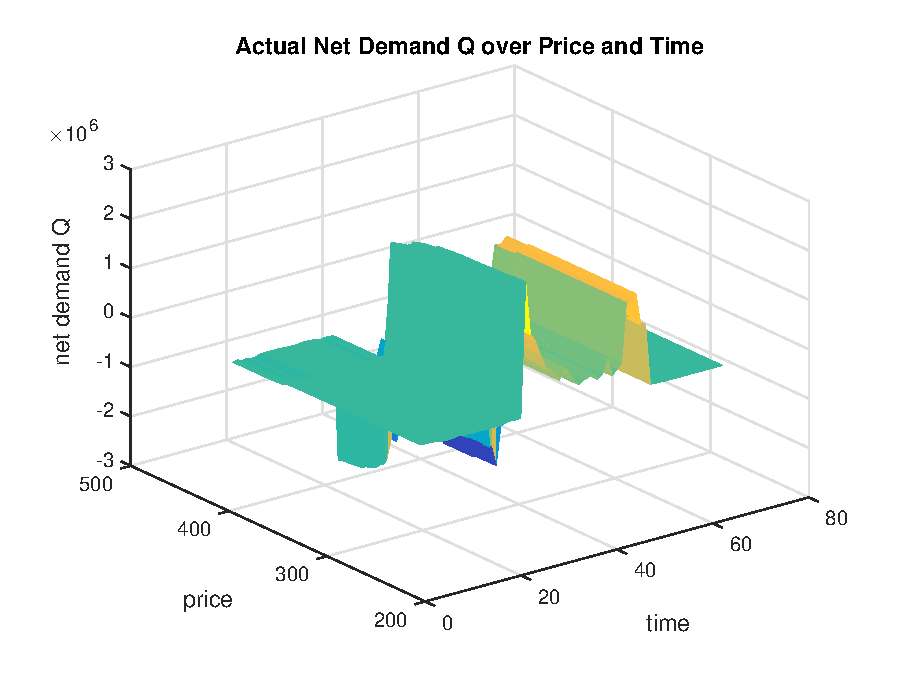
\includegraphics[scale = 0.7]{AAPL_20110401_Calibration_Q.eps}\newline
\caption{The calculated net demand surface $Q$ by price and time, from
market data for AAPL as of April 1st, 2011.}
\label{fig::AAPL_20110401_Calibration_Q}
\end{figure}
\end{center}

After the net demand surface $\hat{Q}$ is calculated, the net demand density
$\hat{q}$ is calculated by taking the first order difference of $\hat{Q}(p)$:

\[
\hat{q}(k,j)=-\frac{\hat{Q}(k,j)-\hat{Q}(k-1,j)}{\Delta p}\text{, \ \  \ \ \
}1\leq k\leq I
\]

Discretization of (\ref{equ_q_A}) yields:%
\[
\hat{h}(k,j)=\frac{1}{\Delta p}(\log (\hat{q}(k,j))-\log {\hat{q}(k-1,j)),}%
\text{ \ \  \ \ \ }2\leq k\leq I
\]%
The net demand elasticity $\hat{\eta}$ is calculated by (\ref{eta}). We
estimate the instantaneous variances by the method of moments:
\begin{eqnarray*}
\hat{\sigma}_{\eta }^{2} &=&\frac{1}{N\Delta t}\sum_{j=-N}^{-1}\frac{\Delta
\hat{\eta}(j)^{2}}{\hat{\eta}(j)(1-\hat{\eta}(j))} \\
\hat{\sigma}_{q}^{2}(1) &=&\frac{1}{N\Delta t}\sum_{j=-N}^{-1}\Delta \hat{q}%
(1,j)^{2} \\
\hat{\sigma}_{h}^{2}(k) &=&\frac{1}{N\Delta t}\sum_{j=-N}^{-1}\Delta \hat{h}%
(k,j)^{2}\text{\ \ \ \ \ \ \ \ \ \ }k=2,...,S
\end{eqnarray*}

We do the same for the instantaneous covariances:%
\begin{eqnarray*}
\hat{s}_{\eta ,q}^{2}(1) &=&\frac{1}{N\Delta t}\sum_{j=-N}^{-1}\Delta \hat{%
\eta}(j)\Delta \hat{q}(1,j) \\
\hat{s}_{\eta ,h}^{2}(k) &=&\frac{1}{N\Delta t}\sum_{j=-N}^{-1}\frac{\Delta
\hat{\eta}(j)\Delta \hat{h}(k,j)}{\sqrt{\eta (j)(1-\eta (j))}}\text{ \ \ \ \
\ \ \ \ \ \ }k=2,...,S \\
\hat{s}_{q,h}^{2}(1,k) &=&\frac{1}{N\Delta t}\sum_{j=-N}^{-1}\Delta \hat{q}%
(1,j)\Delta \hat{h}(k,j)\text{ \ \ \ \ \ \ \ \ \ \ \ \ \ \ \ \ \ }k=2,...,S
\\
\hat{s}_{h}^{2}(k_{1},k_{2}) &=&\frac{1}{N\Delta t}\sum_{j=-N}^{-1}\Delta
\hat{h}(k_{1},j)\Delta \hat{h}(k_{2},j)\text{ \ \ \ \ \ \ \ \ \ \ \ \ \ \ \
\ \ }k_{1},k_{2}=2,...,S
\end{eqnarray*}

We organize the instantaneous variance-covariance matrix as:%
\[
V=\left(
\begin{array}{ccccc}
\hat{\sigma}_{\eta }^{2} & \hat{s}_{\eta ,q}^{2}(1) & \hat{s}_{\eta
,h}^{2}(2) &  & \hat{s}_{\eta ,h}^{2}(I) \\
\hat{s}_{\eta ,q}^{2}(1) & \hat{\sigma}_{q}^{2}(1) & \hat{s}_{q,h}^{2}(1,2)
& \cdots  & \hat{s}_{q_{,}h}^{2}(1,I) \\
\hat{s}_{\eta ,h}^{2}(2) & \hat{s}_{q,h}^{2}(1,2) & \hat{\sigma}_{h}^{2}(2)
& \cdots  & \hat{s}_{h}^{2}(2,I) \\
\vdots  & \vdots  & \vdots  & \ddots  & \vdots  \\
\hat{s}_{\eta ,h}^{2}(I) & \hat{s}_{q_{,}h}^{2}(1,I) & \hat{s}_{h}^{2}(2,I)
& \cdots  & \hat{\sigma}_{h}^{2}(I)%
\end{array}%
\right)
\]%
The factor loading matrix $B$ is the square root of the correlation matrix
corresponding to $V$. It is made of the following coefficients:%
\[
\hat{B}=\left(
\begin{array}{ccccc}
\hat{b}_{\eta }(0) & 0 & \cdots  & \cdots  & \cdots  \\
\hat{b}_{\eta }(1) & \hat{b}_{q}(1,1) & \ddots  &  & \vdots  \\
& \vdots  & \hat{b}_{h}(2,1) & \ddots  & \vdots  \\
& \vdots  & \vdots  & \ddots  & 0 \\
\hat{b}_{\eta }(I) & \hat{b}_{q}(1,I) & \hat{b}_{h}(I,1) & \cdots  & \hat{b}%
_{h}(I,I)%
\end{array}%
\right)
\]

We use Cholesky decomposition to calculate $\hat{B}.$

\bigskip

In the simulation, we use $a_\eta = 0.9$ and $\bar{\eta}=0.6$.


\subsection{Simulation - Real-world Measure ($\mathbb{P}$ Measure)}

The simulated net demand curve under physical measure using the above
methods is shown in left graph of Figure~\ref{fig::AAPL_20110401_simulated_both_measures}.

\begin{center}
\begin{figure}[tbp]
\centering
% Requires \usepackage{graphicx}
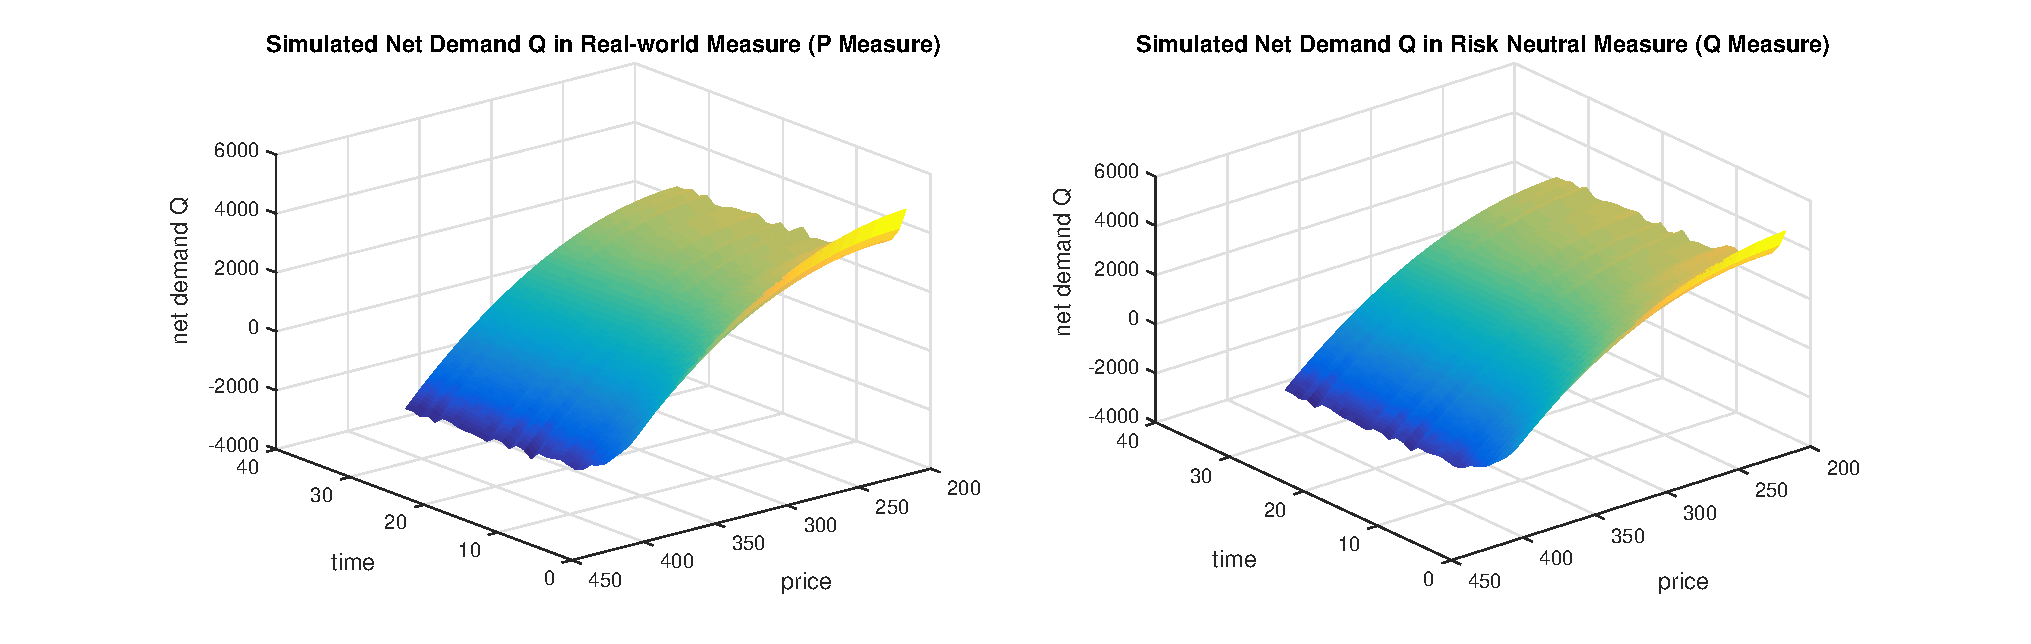
\includegraphics[scale = 0.5]{Q_both_measures.eps}\newline
\caption{The simulated net demand surface Q(p,t) under physical measure
(left) and risk neutral measure (right).}
\label{fig::AAPL_20110401_simulated_both_measures}
\end{figure}
\end{center}

\subsection{Simulation - Risk-Neutral Measure ($\mathbb{Q}$ Measure)}

Let $k^{\ast }(j)$ be the index of the approximate clearing price, i.e., the
value of $k$ that minimizes $|Q(k,j)|$.

We first need to solve the market price of risk equations. Expressions for $%
\mu _{Q}(k,j)$ and $\sigma _{Q}(k,j)$ and $b_{Q}(k,i,j)$ are obtained by
discretization of equations 41 and 42 in the appendix. For more detailed discussion on market price of risk, we refer reader to \cite{NB97}. Remember that:

\[
\Sigma _{Q}(k,i,j)=\sigma _{Q}(k,j)b_{Q}(k,i,j)
\]

We calculate:

\begin{eqnarray*}
\sigma _{\pi }(j)b_{\pi }(i,j) &=&-\frac{\Sigma _{Q}(k^{\ast }(j),i,j)}{%
q(k^{\ast }(j),j)} \\
C(k,j) &=&\sigma _{\pi }(j)\sum_{i=0}^{I}\frac{\Sigma _{Q}(k^{\ast
}(j),i,j)-\Sigma _{Q}(k^{\ast }(j)-1,i,j)}{\Delta p}b_{\pi }(i,j) \\
B(k,j) &=&\mu _{Q}(k,j)-\frac{1}{2}\frac{Q(k+1,j)-2Q(k,j)+Q(k-1,j)}{\Delta
p^{2}}+C(k,j)
\end{eqnarray*}

The market price of risk equations are, for each scenario and each time $j$:

\begin{eqnarray} \label{eqn::market_price_risk_equation}
\sum_{i=0}^{I}\Sigma _{Q}(k,i,j)\lambda (i,j)=B(k,j)\text{ \ \ \ }k=0,...,I
\end{eqnarray}

Now let $\{z^{\mathbb{Q}}(i,j)\}$ be a collection of standard normal random
variates. It remains only to make the substitution:

\[
z(i,j)=z^{\mathbb{Q}}(i,j)\sqrt{\Delta t\Delta s}-\lambda (i,j)\sqrt{\Delta s%
}
\]

in our model (\ref{Euler_1})\ to (\ref{Euler_3}) to obtain the risk-neutral
model.

The simulated net demand surfaces under risk neutral measure is shown in the
right graph of Figure~\ref{fig::AAPL_20110401_simulated_both_measures}. The
range of the difference on net demand (over time and price)
between $\mathbb{P}$-measure simulation and $\mathbb{Q}$%
-measure simulation is $[-50.22,66.10]$ in the case shown in the simulation.

\subsection{Option Pricing}

With the simulations under risk neutral measure, the corresponding call/put
option price, $c(\pi, \omega)$, with strike $K$ at given time $t$ is

\begin{eqnarray*}
c(K) &=& \frac{1}{N} \sum_{\omega} \max\left(\pi(t,\omega)-K,0\right) \\
p(K) &=& \frac{1}{N} \sum_{\omega} \max\left(K - \pi(t,\omega),0\right)
\qquad \omega = 1,2,\ldots,N
\end{eqnarray*}

where $\pi$ is the clearing price at simulation time $t$. With the option
prices, the implied volatility for different strike levels are calculated by
solving

\begin{equation*}
p(K)=BS(\pi ,K,r,T,\sigma (K))
\end{equation*}%
where $BS$ is the Black-Scholes function, $\pi $ is the clearing price, $K$
is the strike level, $r$ is the interest rate, $T$ is time to maturity and $%
p $ is the put option price corresponding to the strike $K$. The implied
volatility $\sigma (K)$ is being solved.

The implied volatility smile generated from the equity options at simulation
period is shown in Figure~\ref{fig::Put_Option_Vols} (right graph). The
implied volatilities by simulations under risk neutral measure are plotted
as blue line, which are compared to the real historical implied volatility
levels from Bloomberg (historical market quotes). The interest rate level
is selected as 0.301\% at real historical level, and the dividend yield
is set to 0\%. The maturity of the option is 60 days. The simulation is
evaluated under 500 scenarios.

The at-the-money simulated implied volatility is within 5\% error range of the Bloomberg
quote, at 25\% level. For low strike options the simulation results tend to
be steeper than the Bloomberg volatility, and the percentage difference
between simulation results and Bloomberg volatilities is within +/- 10\%. As
for the high strike options, the simulation results are flatter than
Bloomberg volatilities.

The left graph in Figure~\ref{fig::Put_Option_Vols} plots the solution of market price
of risk equation \ref{eqn::market_price_risk_equation} ($\lambda(i,j)$) over time, evaluated on at-the-money
price levels. In our simulation process, the market price of risk equation is always solvable through matrix
inversion.

\begin{center}
\begin{figure}[tbp]
\centering
% Requires \usepackage{graphicx}
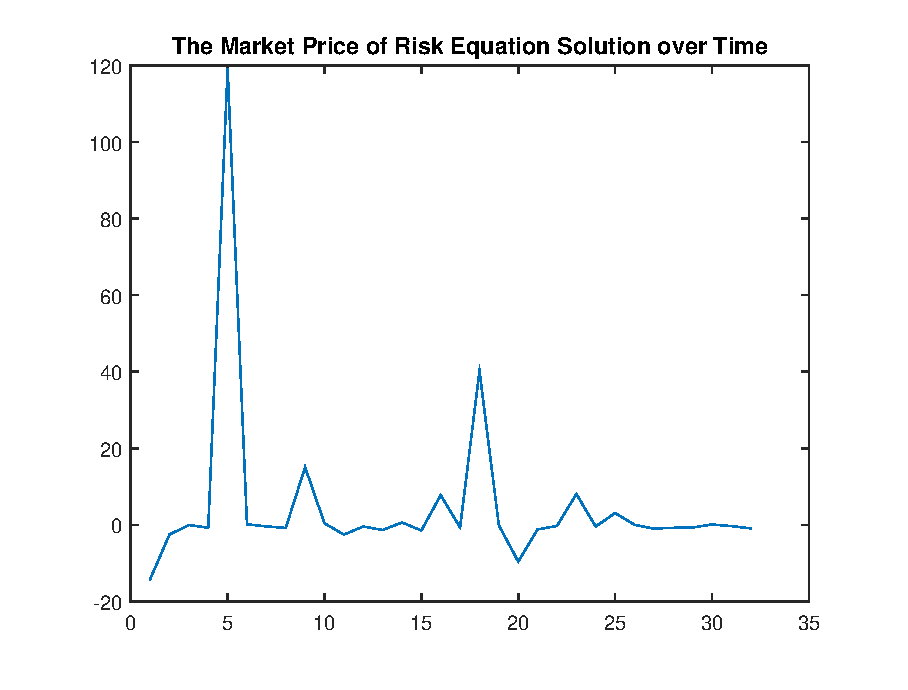
\includegraphics[scale = 0.5]{lambda.eps}
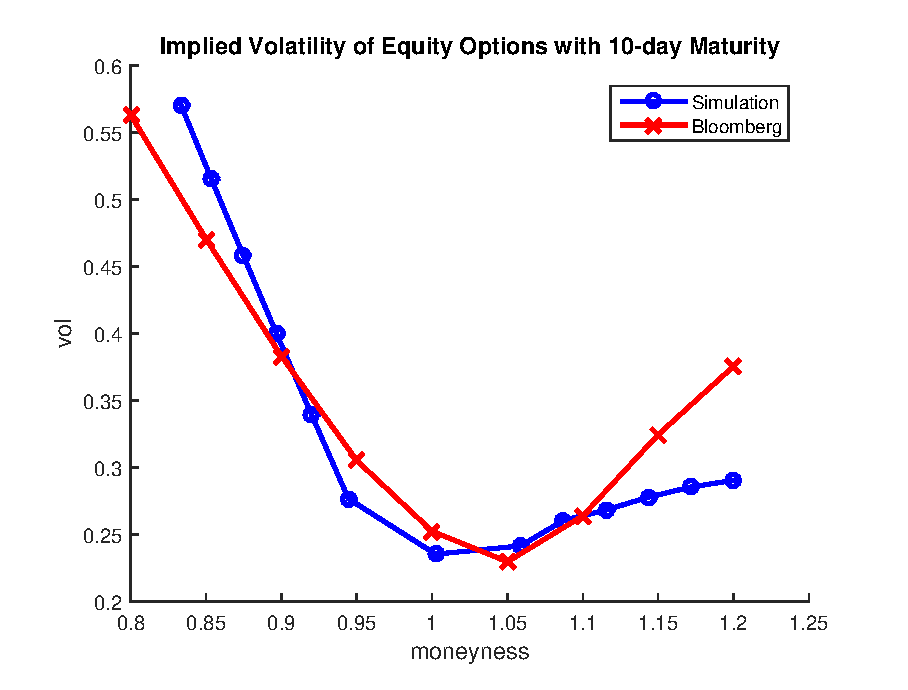
\includegraphics[scale =
0.5]{implied_vol.eps}\newline
\caption{The left graph shows the solution ($\protect\lambda $) of market
price of risk equation at clearing price over time. The right graph plots
implied volatility levels from equity options with maturity of 10 days.}
\label{fig::Put_Option_Vols}
\end{figure}
\end{center}

\appendix
\section{Proof of Proposition}

To prove boundedness in IWK, we will make use of the following elementary
lemma, which is a direct application of the Chebyshev, Cauchy-Schwartz, and
Jensen inequalities.

%\paragraph{Lemma 888}

\begin{lemma}\label{lemma::differentiable_F}
\textit{Let }$Y_{i}(s,t)$\textit{\ and }$Z_{i}(s,t)$\textit{\ be collections
of random variables, for }$i=1,...,n$\textit{, }$0\leq s\leq S$\textit{, and
}$0\leq t\leq T$\textit{. Suppose }$E[\int_{0}^{S}\int_{0}^{T}%
\sum_{i=1}^{n}Y_{i}(s,t)Z_{i}(s,t)ds]<\infty $\textit{. A sufficient
condition for }%
\begin{equation*}
P(\int_{0}^{S}\int_{0}^{T}\sum_{i=1}^{n}Y_{i}(s,t)Z_{i}(s,t)ds<\infty )=1
\end{equation*}

\textit{is that for all }$s,t$\textit{\ and }$i=1,..,n$%
\begin{eqnarray*}
E[Y_{i}(s,t)^{8}] &<&\infty \\
E[Z_{i}(s,t)^{8}] &<&\infty
\end{eqnarray*}
\end{lemma}

In order to prove that some stochastic processes are continuously
differentiable with respect to a parameter $x$, we have the following lemma.

\bigskip

%\paragraph{Lemma 999}

\begin{lemma}\label{lemma::differentiable_F}
Suppose $\int_{0}^{S}b(x,s,t,\omega )^{2}dx=1$. Let
\begin{equation*}
F(x,t,\omega )=\int_{0}^{t}\int_{0}^{S}b(x,s,t,\omega )W(ds,dt,\omega )
\end{equation*}

If $b(.,s,t,\omega )$ is continuously differentiable, then so is $%
F(.,t,\omega )$
\end{lemma}

\paragraph{Sketch of Proof}

we write the quadratic variation of $F$ as:%
\begin{equation*}
\lbrack F(x),F(x)]_{t}=\int_{0}^{t}G(x,S,t)dt
\end{equation*}

where, by a slight abuse of notation, for $s\in \lbrack 0,S]$:

\begin{equation*}
G(x,s,t)=\int_{0}^{s}b^{2}(x,s,t)W(ds,t)
\end{equation*}

Omitting the parameter $t$, $G(x,.)$ has quadratic variation in the $s$
direction given by:%
\begin{equation*}
\lbrack G(x),G(x)]_{s}=\int_{0}^{s}b^{2}(x,s)ds
\end{equation*}

Since $[G(x),G(x)]_{s}$ is continuously differentiable in $s$, by theorem
3.1.2 in Kunita $G(x,s,t)$ is differentiable in $x$. Thus $[F(x),F(x)]_{t}$
is continuously differentiable in $p$. Applying 3.1.2 in Kunita again, the
result obtains.

\subsection{Preliminaries}

Differentiating (\ref{equ_Q_A}), we have:

\begin{eqnarray}
\frac{\partial Q(p,t)}{\partial p} &=&-\exp \left( {\int_{x=0}^{p}h(x,t)dx}%
\right)   \label{dQdp_3} \\
\frac{\partial ^{2}Q(p,t)}{\partial p^{2}} &=&-{h(p,t)}\exp \left( {%
\int_{x=0}^{p}h(x,t)dx}\right)   \label{dQdp_2_3}
\end{eqnarray}

As for the infinitesimal parameters of $Q$, let:%
\begin{eqnarray}
f(p,t) &=&\int_{x=0}^{p}{h(x,t)}\exp ({\int_{x=0}^{x}h(x,t)dx)}a(p)(\bar{h}%
(p)-x)dx  \label{f_of_p} \\
&&\frac{1}{2}\int_{x=0}^{p}\text{ }{h}^{2}{(x,t)}\exp ({%
\int_{x=0}^{x}h(x,t)dx)}\sigma _{h}^{2}(x)dx+  \notag \\
&&\frac{1}{2}({h(p,t)}\exp ({\int_{x=0}^{p}h(x,t)dx)}\sigma _{h}^{2}(p)|-{%
h(0,t)}\sigma _{h}^{2}(0))  \notag \\
&&\frac{1}{2}\int_{x=0}^{p}{h(x,t)}\exp ({\int_{y=0}^{x}h(y,t)dx)[h(x,t)}%
\sigma _{h}^{2}(x)+\frac{d}{dx}\sigma _{h}^{2}(x)]dx  \notag
\end{eqnarray}

By Ito's lemma, the drift of $Q(p,t)$ is:%
\begin{eqnarray}
\mu _{Q}(p,t) &=&\eta (t)f(S,t)-f(p,t)+  \label{mu_Q} \\
&&a_{\eta }(\bar{\eta}-\eta (t))\int_{x=0}^{S}\exp ({%
\int_{y=0}^{x}h(y,t)dy)dx+}  \notag \\
&&g(\eta (t))\int_{x=0}^{S}{h(x,t)}\exp ({\int_{y=0}^{x}h(y,t)dy)\sigma
_{h}(x)dx}  \notag
\end{eqnarray}

while the volatility of $Q(p,t)$ is:%
\begin{eqnarray}
\sigma _{Q}(p,t)b_{Q}(p,s,t) &=&g(\eta (t))b_{\eta }(s)(Q(S,t)-Q(0,t))+
\label{sigma_Q} \\
&&\eta (t)\int_{x=0}^{S}{h(x,t)}\exp ({\int_{y=0}^{x}h(y,t)dy)}\sigma
_{h}(x)b_{h}(x,s)dx-  \notag \\
&&\int_{x=0}^{p}{h(x,t)}\exp ({\int_{y=0}^{x}h(y)dy)}\sigma
_{h}(x)b_{h}(x,s)dx  \notag
\end{eqnarray}

\subsection{Verification of Assumptions~\ref{ass::demand_twice_diff} and~\ref{ass::iwk_condition_Q}}

It is clear from (\ref{dQdp_2_3}), and lemma 999 that $Q$ is twice
continuously differentiable in $p$. Thus assumption 4 is satisfied as well
as IWK (ii)\ (continuity of $Q$ in $p$)

Assumption IWK (i) (boundedness of $P(t)$) is verified in remark x..

\subsubsection{Verification of IWK iii.a)}

Drift:\ As seen above $h(p,t)$ is continuous in $p$.  By continuity of $a(p)$
and $\frac{d}{dp}\sigma _{h}^{2}(p)$ the process $f(p,t)$ is differentiable
in $p$. Inspection of (\ref{mu_Q}) shows that $\mu _{Q}$ is continuous in $p$%
.

Volatility: We need only investigate the third row of (\ref{sigma_Q}), which
is clearly a continuous function of $p$. So is $\sigma _{Q}(p,t)$.

\bigskip

\subsubsection{Verification of IWK iii.b)}

Continuity of (1)\ and (2) obvious. From (\ref{sigma_Q}), we calculate
\begin{equation}
\frac{\partial \lbrack \sigma _{Q}(p,t)b_{Q}(p,s,t)]}{\partial p}=-{%
h(p,t,\omega )}\exp ({\int_{x=0}^{p}h(x,t)dx)}\sigma _{h}(p,t)b_{h}(p,s,t)
\label{dsigmadp}
\end{equation}

which is clearly a continuous function of $p$, thus proving continuity of
(3). Continuity of (4) and (5) follows trivially.

\subsubsection{Verification of IWK iv and v}

Clearly ${\int_{y=0}^{p}h(y,t)dy}$ is normal, thus $q(p,t)$ is lognormal,
and has thus finite moments. For simplicity, we drop the argument $t$. By
Lemma~\ref{lemma::differentiable_F}, we can break the argument into verifying finiteness of the 16th
moments of the following random variables:

\begin{enumerate}
\item \textbf{Net demand\ }$Q(p).$ By Jensen's inequality:%
\begin{equation*}
E[(\int_{0}^{S}q(x)dx)^{16}]\leq \int_{0}^{S}E[\exp (16\int_{0}^{x}h(y)dy)]ds
\end{equation*}%
which is bounded. By (\ref{equ_Q_A})
\begin{equation*}
-\int_{x=0}^{S}q(x)dx\leq Q(p)\leq \int_{x=0}^{S}q(x)dx
\end{equation*}

Thus $E[Q(p)^{16}]$ is bounded.

\item \textbf{Volatility of net demand }$\sigma _{Q}$.  Observe that $\sigma
_{h}(x,s)$ is bounded. Since $g(\eta )$ and $\eta $ are bounded, it suffices
to look at the last term of (\ref{sigma_Q}), to which we apply Jensen's
inequality:%
\begin{gather*}
E[(\int_{x=0}^{S}{h(x)}\exp ({\int_{y=0}^{x}h(y)dy)}dx)^{16}]=E[(%
\int_{x=0}^{S}\frac{d}{dx}\exp ({\int_{y=0}^{x}h(y)dy)}dx)^{16}]= \\
E[\exp ({\int_{y=0}^{S}h(y)dy)}dx)^{16}]
\end{gather*}

Thus $E[\sigma _{Q}(p)^{16}]$ is bounded.

\item \textbf{Drift of net demand }$\mu _{Q}.$Applying Jensen's inequality
and the Cauchy-Schwartz inequalities to (\ref{mu_Q}), it is sufficient to
verify the finiteness of the 16th moments of:

$f(S),\int_{x=0}^{S}\exp ({\int_{y=0}^{x}h(y)dy)dx}$, and $\int_{x=0}^{S}{%
h(x)}\exp ({\int_{y=0}^{x}h(y)dy)\sigma _{h}(x)dx}$. For $f(S)$, the same
type of development applies for the first 3 terms. $E[f(S)^{16}]$ is bounded
because$\sigma _{h}^{2}(x)$ is differentiable.

\item \textbf{Price drift }$\mu _{P}.$We refer the reader to (\ref{mu_Px}) in
the main text. Since the numerator has finite 16th moment, it is sufficient,
by the Cauchy-Schwartz inequality, to prove boundedness of:%
\begin{equation*}
E[(\frac{1}{\partial Q/\partial p})^{16}]=E[\exp \left( -16{%
\int_{x=0}^{p}h(x,t)dx}\right) ]
\end{equation*}%
\qquad which is obvious.

\item \textbf{Price volatility }$\sigma _{P}:$We use the same argument as
above, since%
\begin{equation*}
\sigma _{P}=\frac{\sigma _{Q}}{\partial Q/\partial p}
\end{equation*}

\item \textbf{First derivative of net demand} $\frac{\partial Q(p)}{\partial
p}$Finiteness of the moment is clear, since the random variable in (\ref%
{dQdp_3}) is lognormal.

\item \textbf{Second Derivative of Net Demand}$\frac{\partial Q^{2}(p)}{%
\partial p^{2}}$

Using Cauchy-Schwartz on (\ref{dQdp_2_3}), we see that this has finite
appropriate moment.

\item \textbf{Derivative of Net Demand Volatility }$\frac{\partial \sigma
_{Q}(p)b_{Q}(p,s)}{\partial p}$

We reuse (\ref{dsigmadp}), and use the same logic as above.
\end{enumerate}

\subsection{Verification of Assumption~\ref{ass::iwk_condition_P}}

Since $Q(.,t)$ is bijectiveand continuous, so is its inverse $P(.,t)$. Thus
IWK (ii) is verified. We rewrite (\ref{dQdp_3}) as:

\begin{equation*}
\frac{\partial Q(P(x,t),t)}{\partial p}=-\exp \left( {%
\int_{x=0}^{P(x,t)}h(y,t)dy}\right)
\end{equation*}

Thus:%
\begin{eqnarray}
\frac{\partial P(x,t)}{\partial x} &=&-\exp \left( {%
\int_{x=0}^{-P(x,t)}h(y,t)dy}\right)   \label{dPdx} \\
\frac{\partial ^{2}P(x,t)}{\partial x^{2}} &=&P(x,t)\exp \left( {%
\int_{x=0}^{-P(x,t)}h(y,t)dy}\right)   \label{dPdx_square}
\end{eqnarray}

\subsubsection{Verification of IWK iii.a) }

Immediate from (\ref{mu_Px}),(\ref{sigma_P})\ and (\ref{b_P}). Continuity of
the parameters of $Q$ was proved under assumption 7

\bigskip

\subsubsection{Verification of IWK iii.b)}

Continuity of (1)\ and (2) obvious. From (\ref{sigma_P}), we calculate
\begin{equation}
\frac{\partial \lbrack \sigma _{P}(x,t)b_{P}(x,s,t)]}{\partial x}=-\frac{%
\partial }{\partial x}\left( \frac{b_{Q}(P(x,t),s,t)\sigma _{Q}(P(x,t),s,t)}{%
\frac{\partial Q}{\partial p}(P(x,t))}\right)   \label{dsigmadp}
\end{equation}

and continuity follows from the differentiability of $P$ (see \ref{dPdx}).

\subsubsection{Verification of IWK iv and v}

For simplicity, we drop the argument $t$. By Lemma~\ref{lemma::differentiable_F}, we can break the
argument into verifying finiteness of the 16th moments of the following
random variables:

\bigskip

\begin{enumerate}
\item \textbf{Price }$P(x).$ By definition it is bounded.

\item \textbf{Volatility of price }$\sigma _{P}$. Obvious from the proof of
Assumption~\ref{ass::iwk_condition_Q}.

\item \textbf{Price drift }$\mu _{P}.$Obvious from the proof of Assumption~\ref{ass::iwk_condition_Q}.

\item \textbf{Strategy drift }$\mu _{\theta }.$ By Assumption~\ref{ass::theta_semimartingale}.

\item \textbf{Strategy volatility }$\sigma _{\theta }$ By Assumption~\ref{ass::theta_semimartingale}.

\item \textbf{First derivative of price} $\frac{\partial P}{\partial x}$
From (\ref{dPdx}).

\item \textbf{Second derivative of price}$\frac{\partial ^{2}P}{\partial
x^{2}}$ From (\ref{dPdx_square}).

\item \textbf{Derivative of Price Volatility }$\frac{\partial \lbrack \sigma
_{P}(x,t)b_{P}(x,s,t)]}{\partial x}$From (\ref{dsigmadp}).
\end{enumerate}

\subsection{Verification of Assumption~\ref{ass::novikov_condition_lambda} and Equation (\protect\ref{MPR})}

We first verify that $B(p,t)$ is differentiable in $L^{2}(\mathbb{P})$. The
term $\frac{\partial ^{2}Q}{\partial p^{2}}$ is differentiable in $p$ by
Lemma~\ref{lemma::differentiable_F}. A similar line of proof allows us to conclude (see also the proof
of assumption 1) that $\mu _{Q}(p,t)$ and $C(p,t)$ are also differentiable.
Thus $B(p,t)$ is differentiable. We now differentiate the MPR w.r.t. $p$ to
obtain:%
\begin{equation*}
\int_{\delta _{1}}^{S}{h(p,t)}\exp ({\int_{y=0}^{p}h(y)dy)}\sigma
_{h}(p)b_{h}(p,s)\lambda (s)ds=\frac{\partial B(p)}{\partial p}\text{ }
\end{equation*}

Since ${h(p,t)}$ is different from zero by probability one, we have, for $%
p\in \lbrack 0,S]$:%
\begin{equation}
\int_{\delta _{1}}^{S}b_{h}(p,s)\lambda (s)ds=\frac{\frac{\partial B(p)}{%
\partial p}}{{h(p,t)}\exp ({\int_{y=0}^{p}h(y)dy)}\sigma _{h}(p)}
\label{tobeinverted}
\end{equation}

where the right-hand side is a.s. bounded (see the proof of Assumption~\ref{ass::market_frictionless}). By
the assumption that $B_{h}$ has full rank, $\lambda (s)$ is determined by (%
\ref{tobeinverted}) for $s\in \lbrack \delta _{1},S]$, and is a.s. bounded.
We can then specify $\lambda (s)$ for $s\in \lbrack 0,\delta _{1}]$ by
solving the single equation:

\begin{equation}
\int_{s=0}^{\delta _{1}}\Sigma (0,s)\lambda (s)ds=B(0)-\int_{s=\delta
_{1}}^{S}\Sigma (0,s)\lambda (s)ds  \label{this}
\end{equation}

Since the right-hand side is a.s bounded, it is possible to find a solution $%
\lambda (s)$ to (\ref{this}) for $s\in \lbrack 0,\delta _{2}]$ which is a.s.
bounded. By Theorem 7.19 in DPZ, Novikov's criterion holds.


\bibliographystyle{plain}
\bibliography{bib}

\end{document}
